\section{Trash Robot}

\subsection{What is Trash Robot?}

Everything here refers back to Ontology.  We build this thing, show how to replicate it, show how replication can benefit the replicator, which stimulates further replication.  Build things and sell them. Build things and use them. Build things and share them for mutual aid and benefit. 

Metabusiness.  SRS.  Thing.  Organic Media. Geometron vehicle.  Maker swarm. Methodology.  Trash Magic(self replicating media from trash, seed of full complete set).

The Street Network can be used to sell a huge range of goods and services.  Trash Robot is a specific collection of self-replicating technologies which can also be sold directly via the Street Network.  It includes a list of things which will be described here, which readers are encouraged to copy and sell.  But more importantly it provides a prototype for a new type of product which can be built at scale using the decentralized craft mode of production.  As soon as this book is released and we build a swarm to start living Geometron and selling the elements of Trash Robot and bartering for the services provided by the Network we will also start building totally new products using this method.  We will work to build products which have not exact equivalent on the market in the consumer economy and which would be very difficult to replicate in that space for various logistical reasons of how technology scales.   IN particular we need to explore in this chapter the economics of enclosures and how cardboard and duct tape and geometron built by crafters and immediately sold at a profit on a one-at-a-time basis differs from injection molding of enclosures at scale.  

\subsection{The Open Brand}

rainbow and googly eyes.  Soft black textiles. Felt.  Geometric constructions from Geometron.  Use of geometry in cardboard fabrication, HDPE sheets. Modularity.  Things carried in cloth bags. Blocky geometric font.  duct tape and cardboard and sticks. Things built from trash.  Images of the things: box, flag, shirt, pants, bags with robots.  The fashion brand.  

\subsection{The ArtBox}

As with everything in Trash Robot the ArtBox is a self-replicating set.  The elements are the Trash Ties, the Tape Snake, a purse which is the box itself, and a collection of standard art supplies which sit in the box and are used to make another box.  Trash Ties are 6 foot long sections of cotton clothesline, with the ends duct taped.  We buy a whole package of 100 feet of clothesline, and cut into 6 foot sections, duct taping where the cut will be before cutting so each section has both ends taped.  We then buy a collection of colored duct tapes which includes black, red, orange, yellow, green, blue, purple, and pink, or one more if it is available.  We thread the Trash Tie through all of them twice, and join it to itself with a square knot.  This is the Tape Snake.  We carry this around with us to anyplace where we are working on replication. 

The contents of the box are box cutters, sharpie markers, a laser cut acrylic shape set as documented elsewhere in this chapter, and a bag of googly eyes(which can be purchased in bulk online for very little money), scissors, and a ruler, also documented elsewhere here.


\begin{figure}
	\centering
	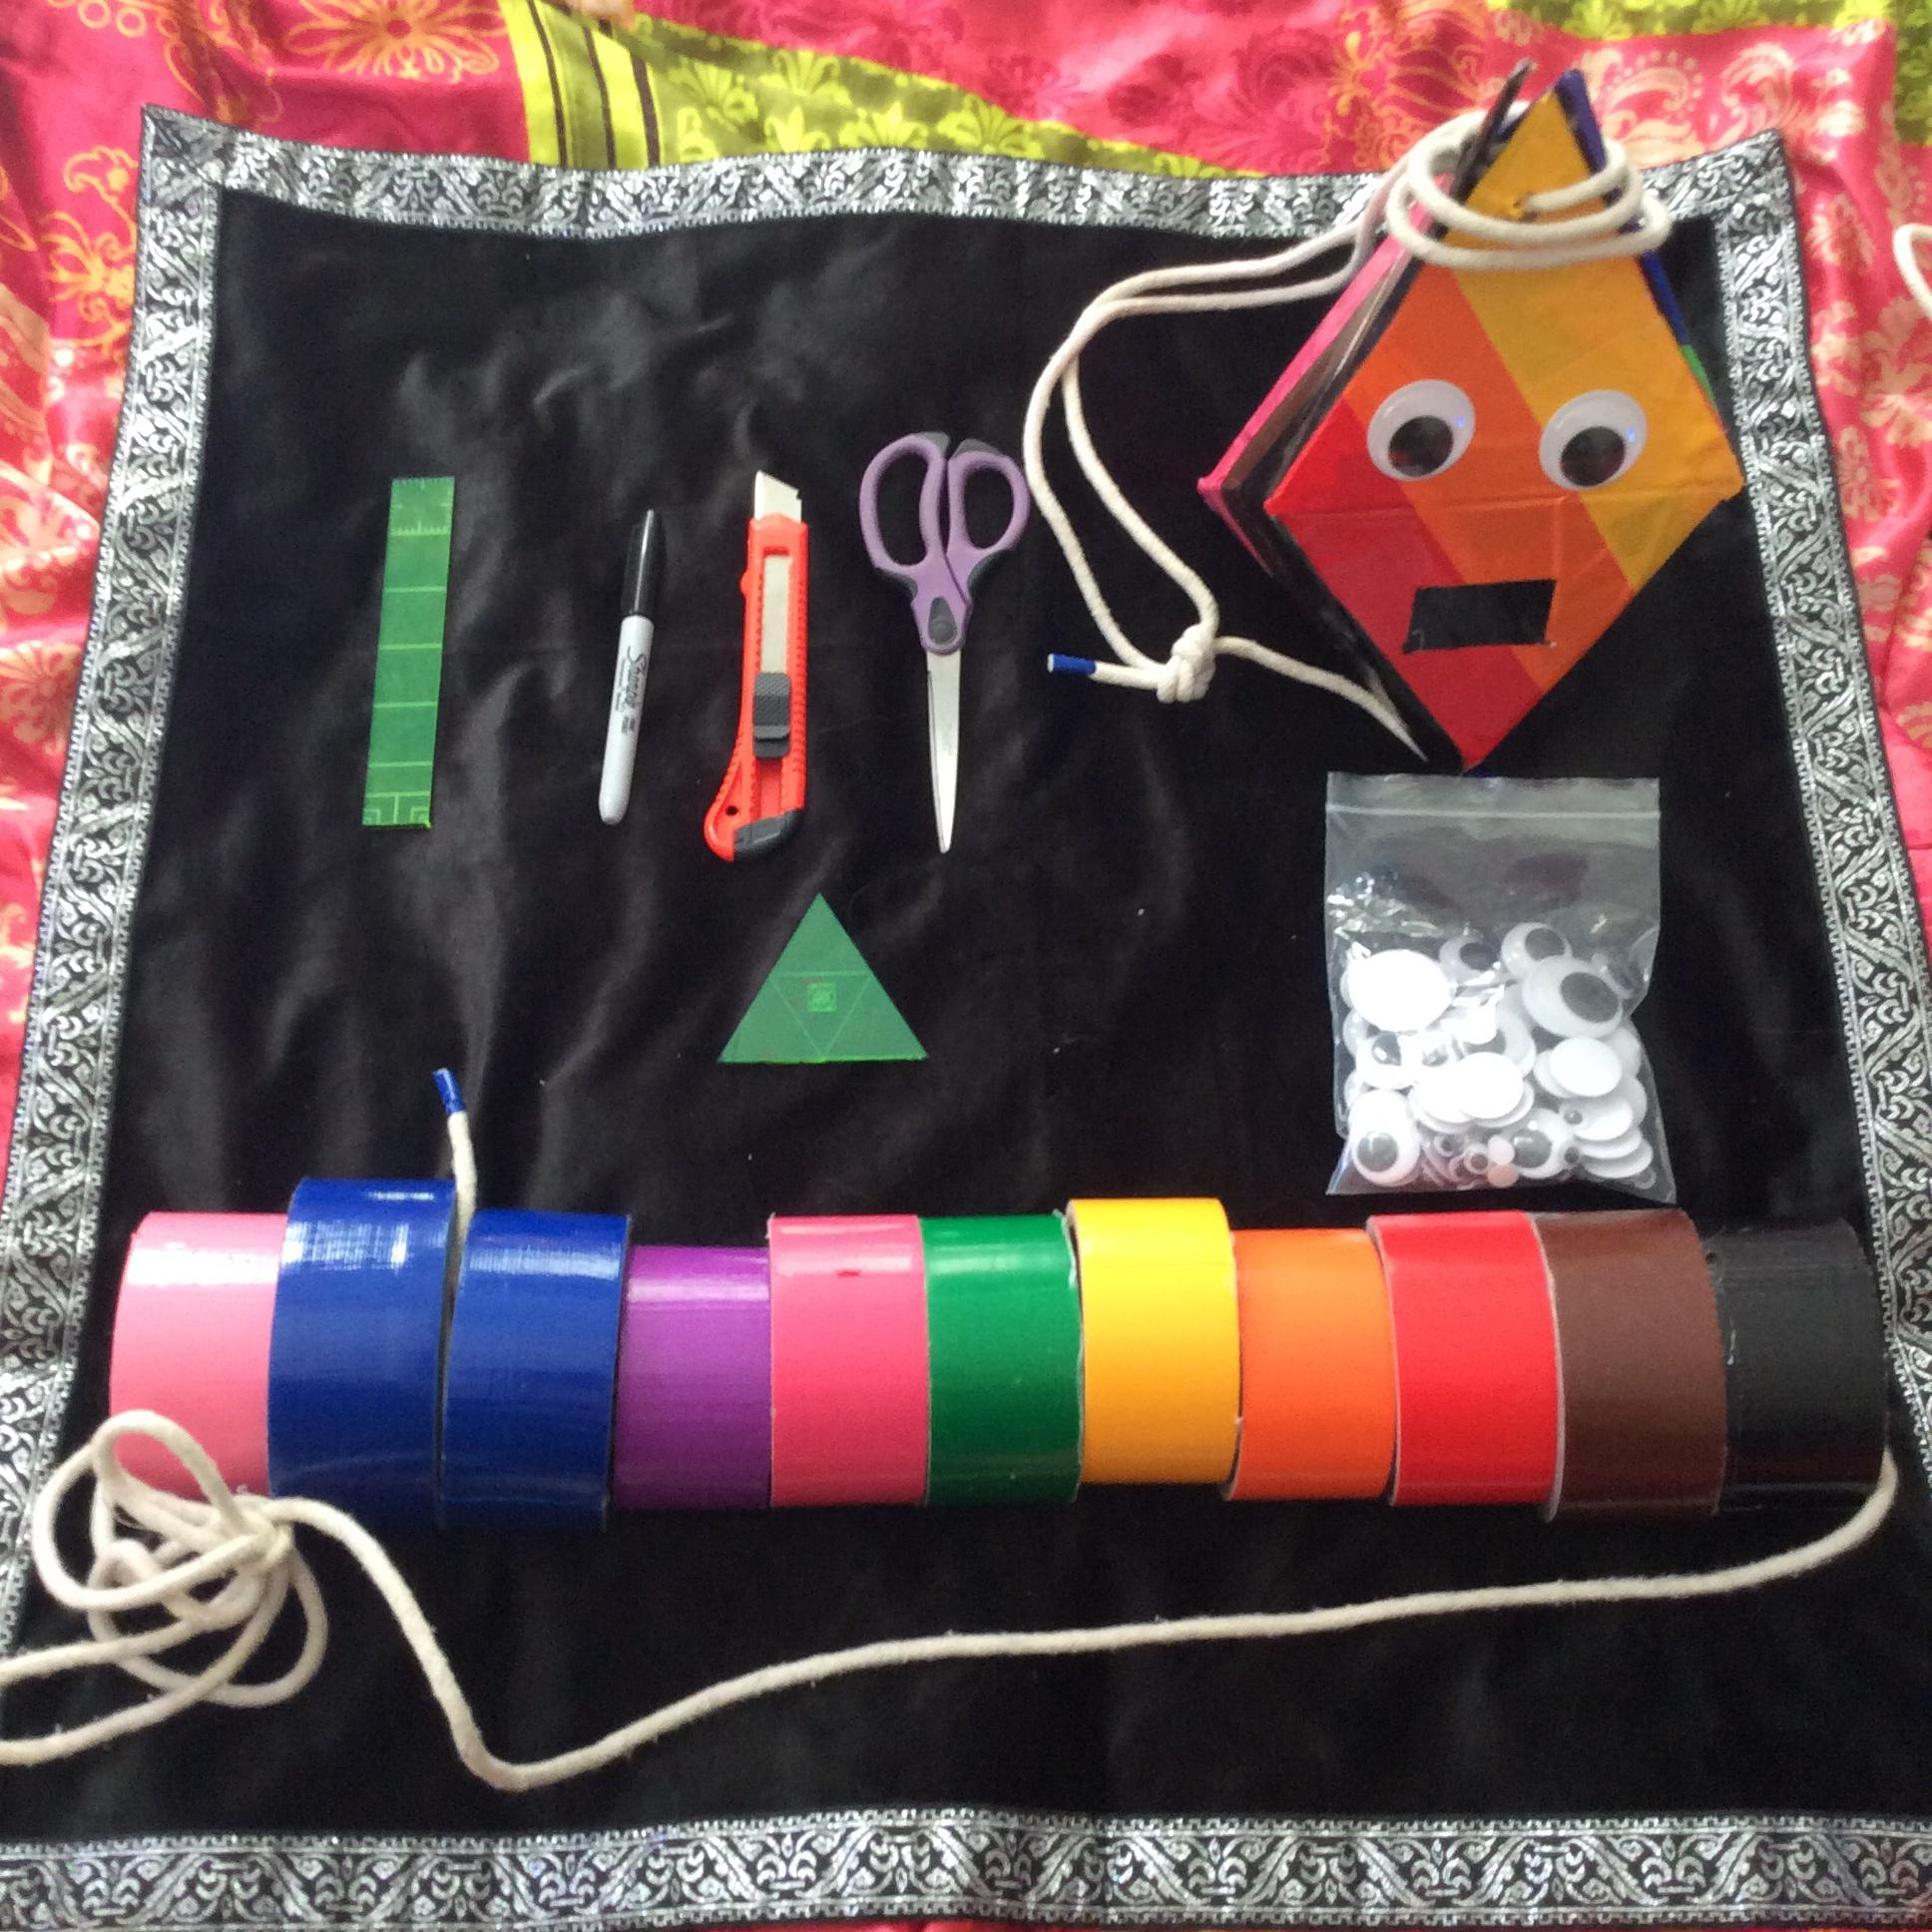
\includegraphics[width=4in]{figures/artboxelements.jpg}
	\caption[artboxelements]
	{Elements of the ArtBox and a Tape Snake.}
\end{figure}


This is a nice purse! If you make one and have the supplies you can go make one with a friend and they can make more and so on.  And as you all make them and grow the swarm you can use them to carry around art supplies for other art projects as a super stylish art supplies purse until people notice and want to buy it, then a market will exist and we will sell them to whoever wants them.  These are so striking and nice to use and cost so little to make and are so easy to copy that they can be a big part of what replicates the whole Trash Robot system which in turn helps replicate all of Geometron and the Street Network.


\begin{figure}
	\centering
	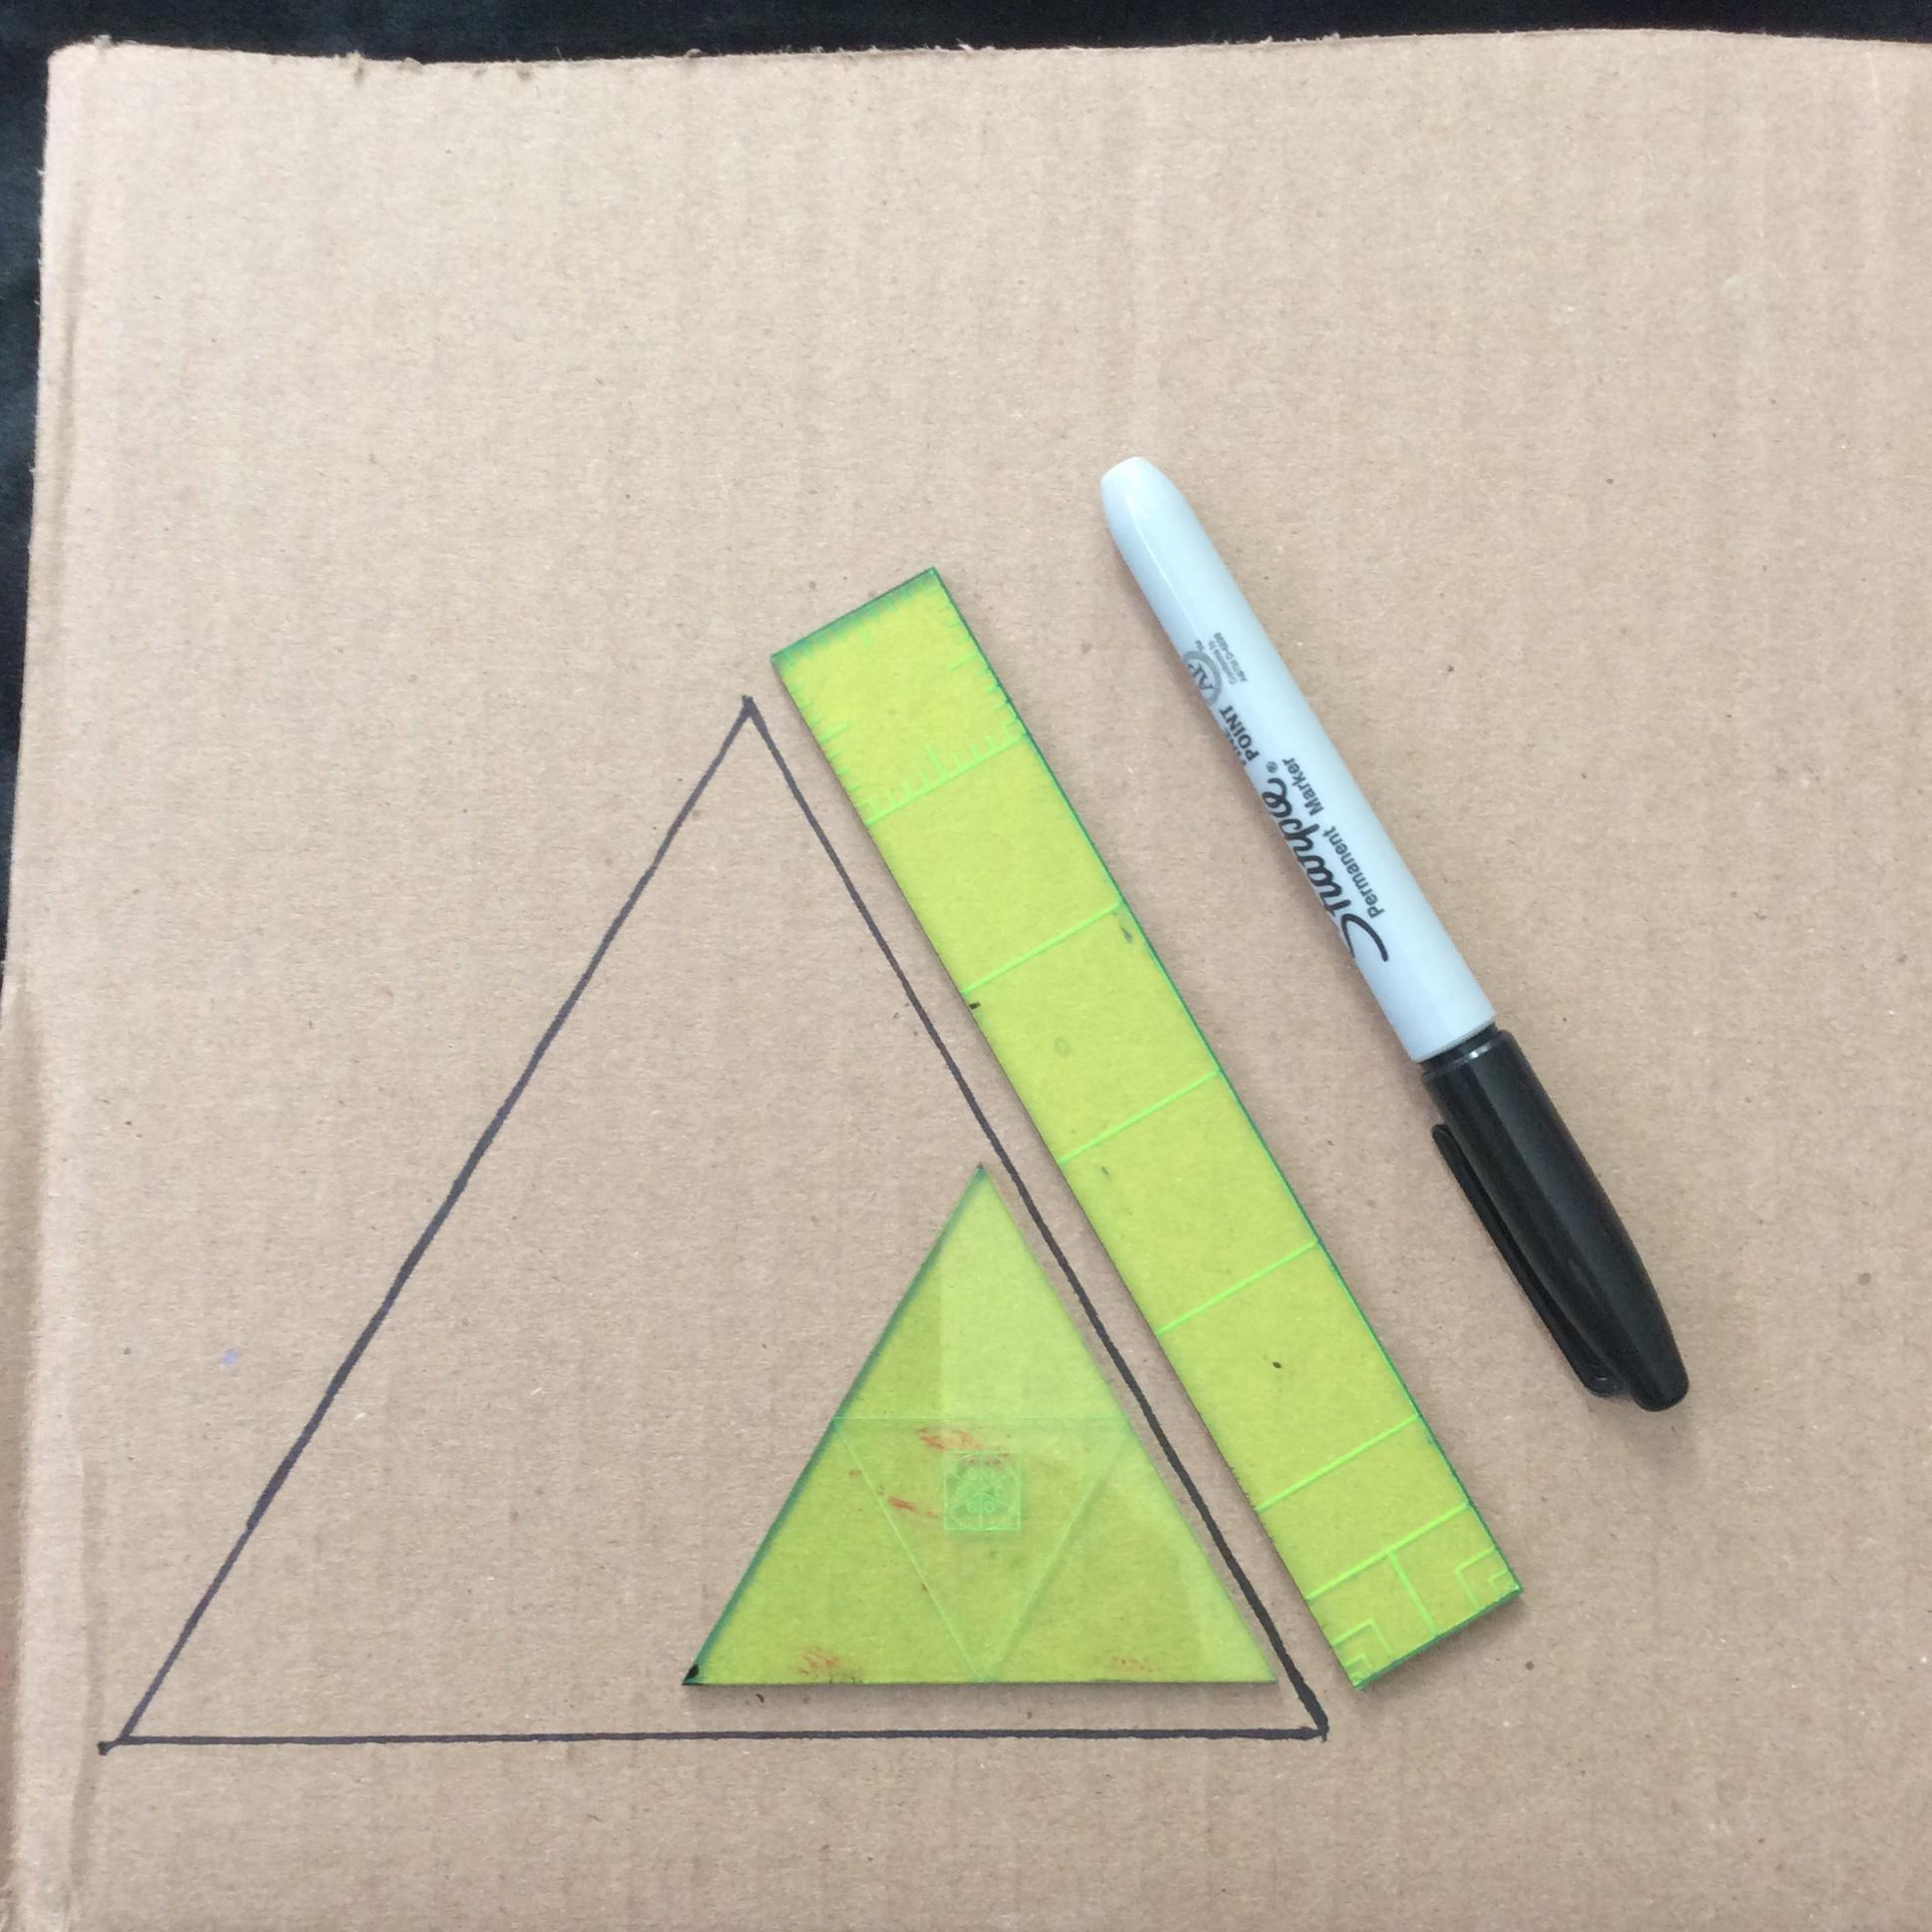
\includegraphics[width=4in]{figures/artboxtriangle.jpg}
	\caption[artboxtriangle]
	{Cut out a 6 inch equilateral triangle from thick corrugated cardboard.}
\end{figure}

\begin{figure}
	\centering
	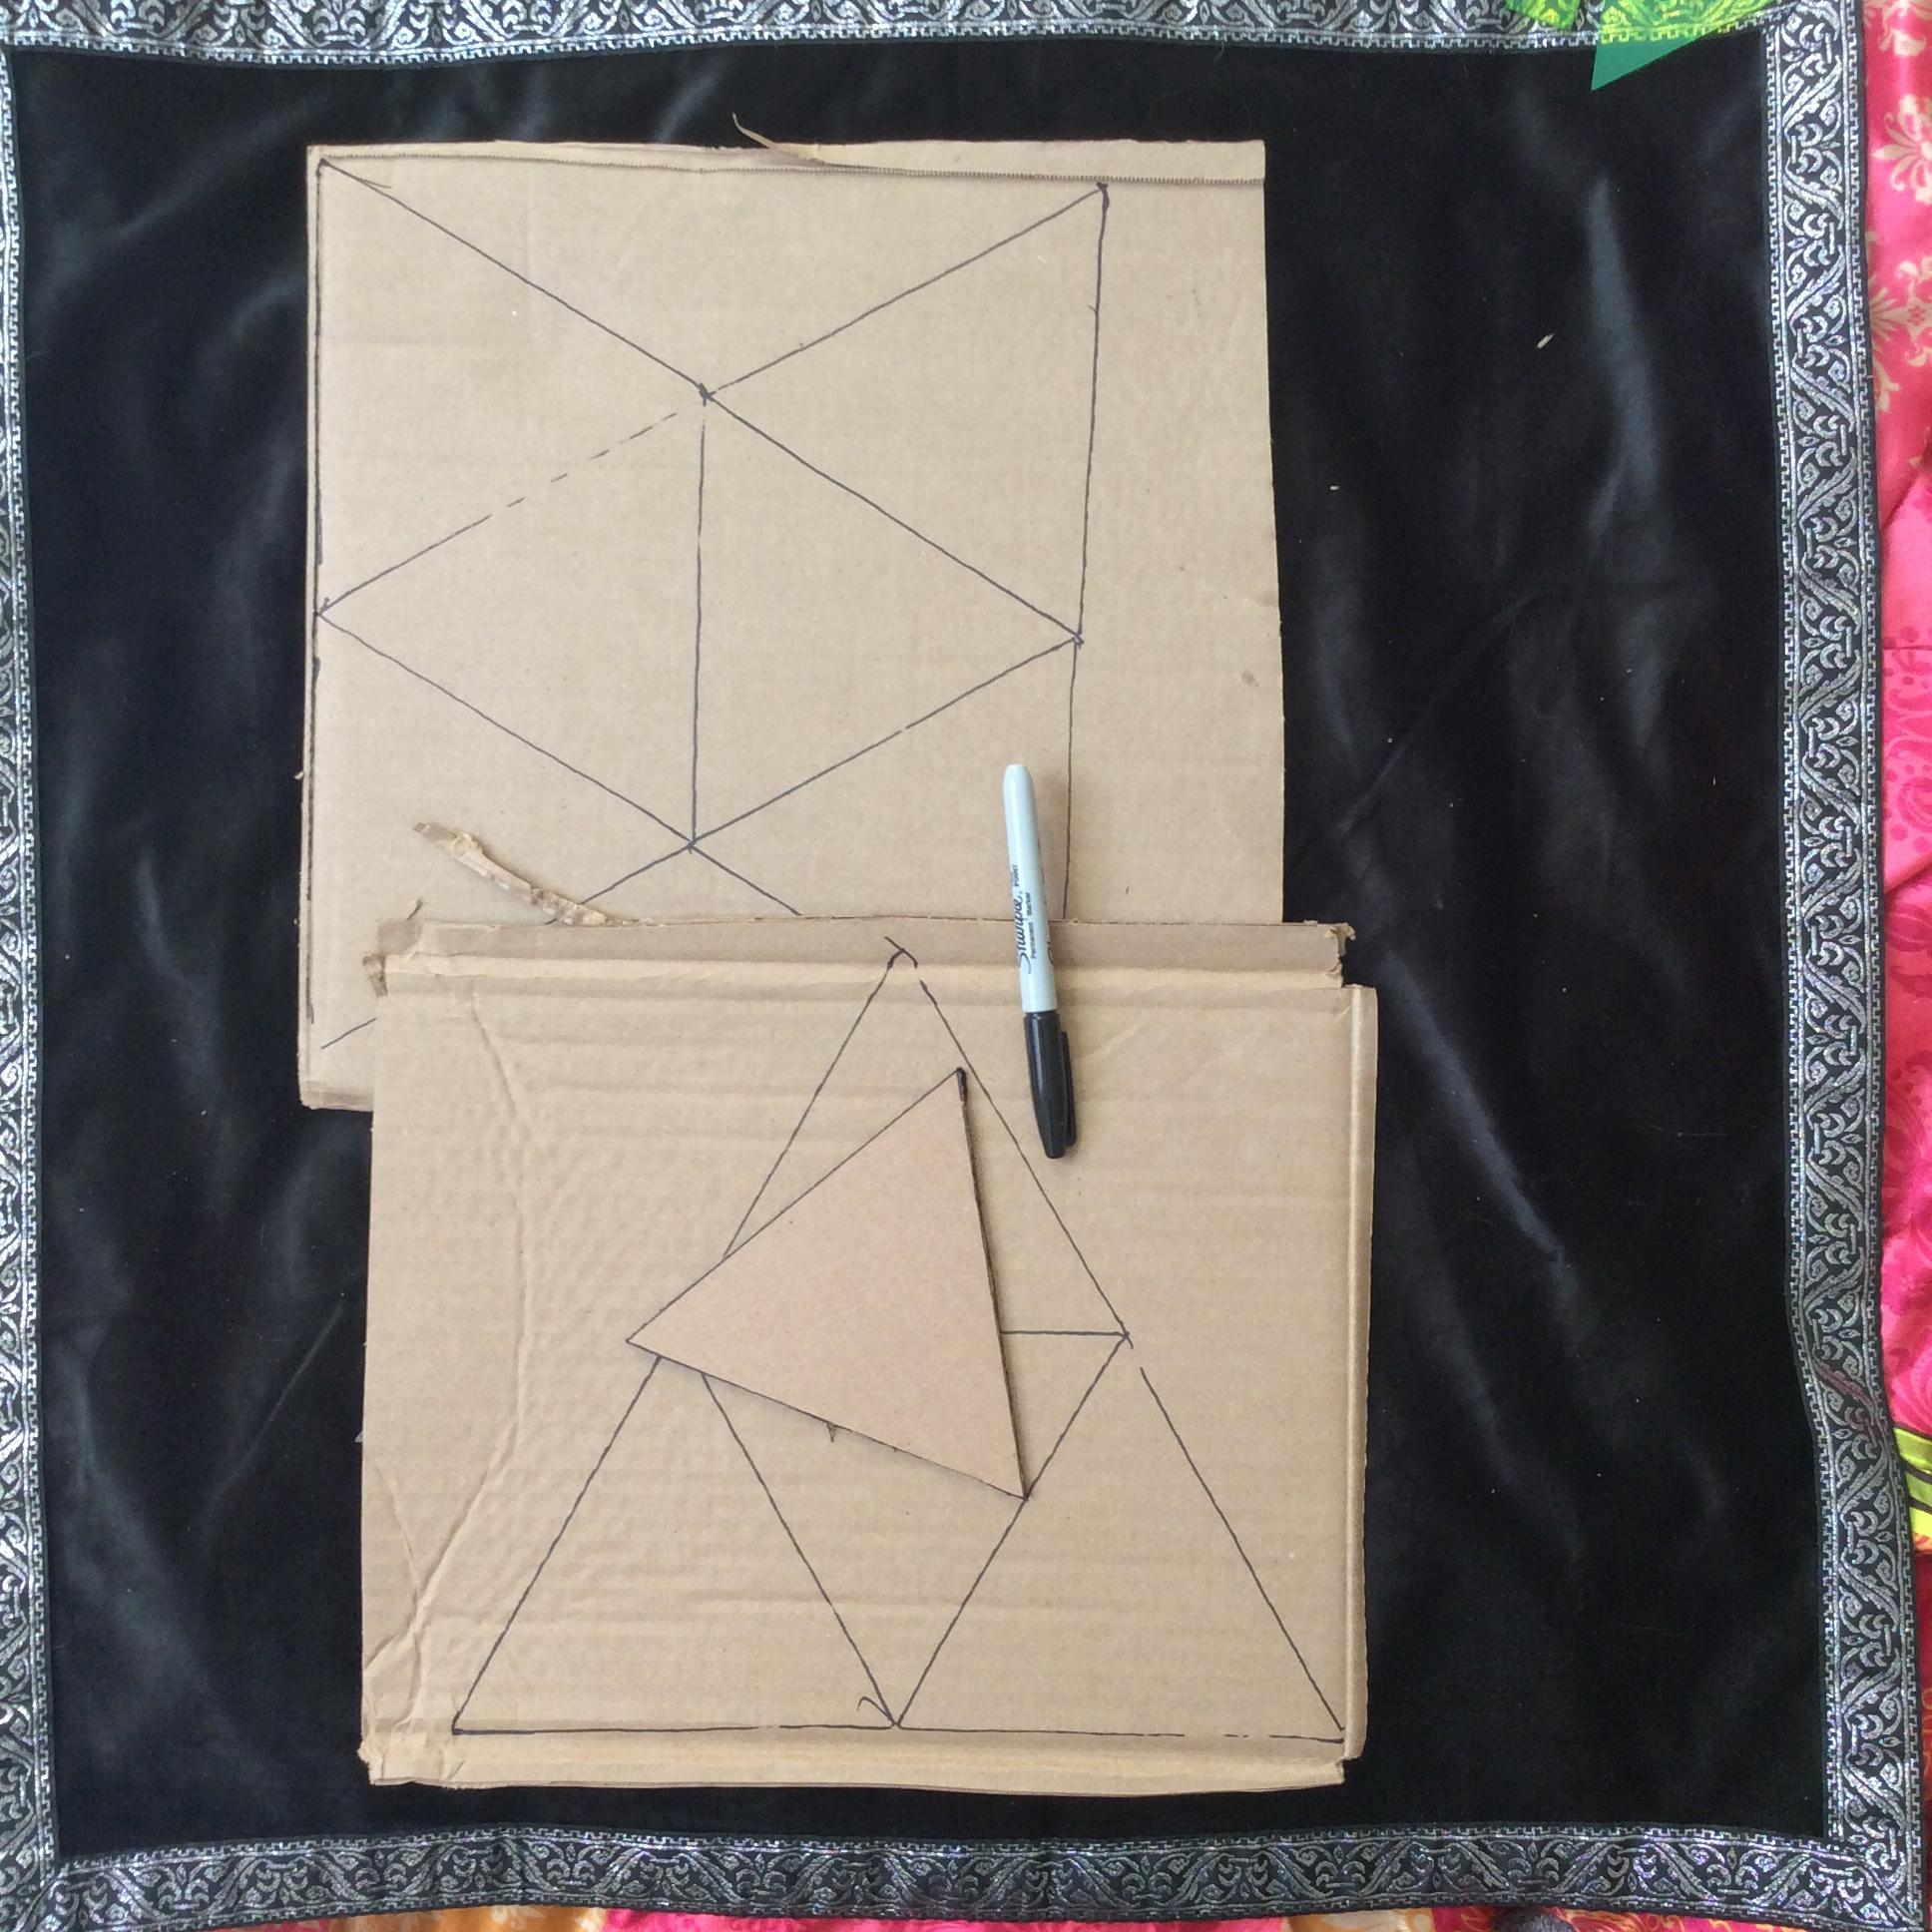
\includegraphics[width=4in]{figures/artboxtriangleset.jpg}
	\caption[artboxtriangle]
	{Copy so that you have a total of 10 triangles.}
\end{figure}

\begin{figure}
	\centering
	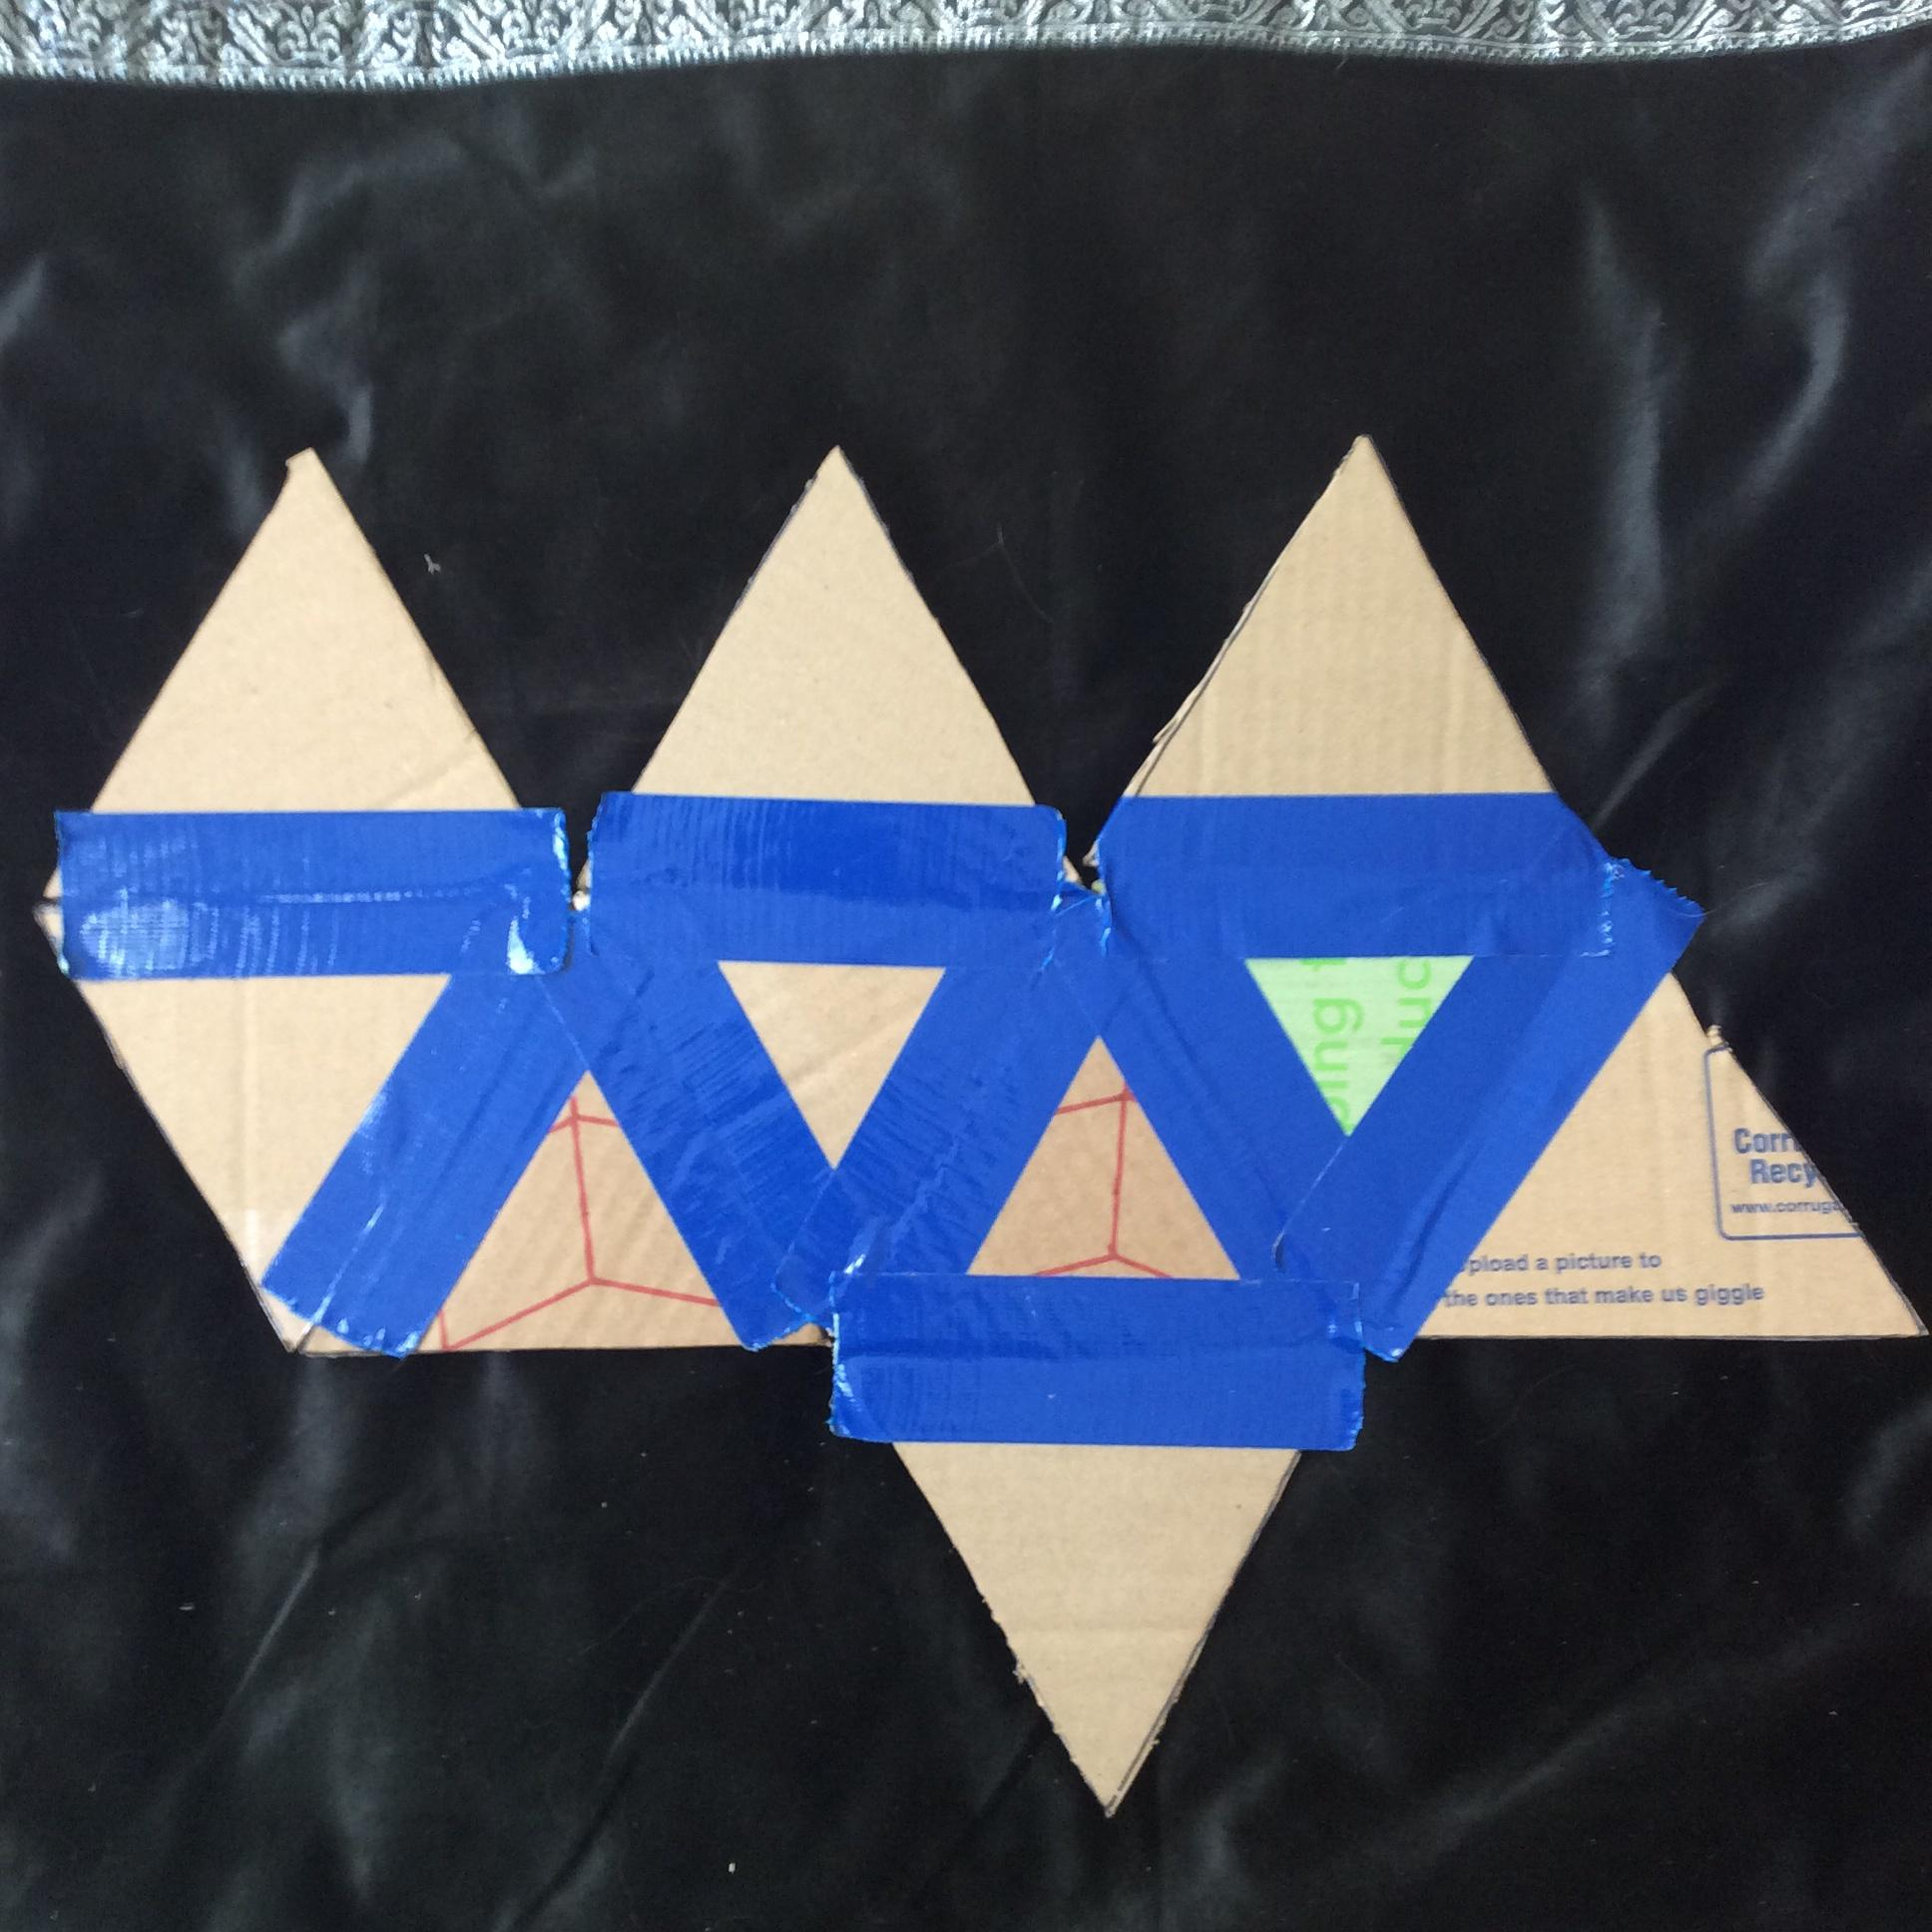
\includegraphics[width=4in]{figures/artboxnet.jpg}
	\caption[artboxtnet]
	{Stitch together the net pattern as shown.}
\end{figure}


\begin{figure}
	\centering
	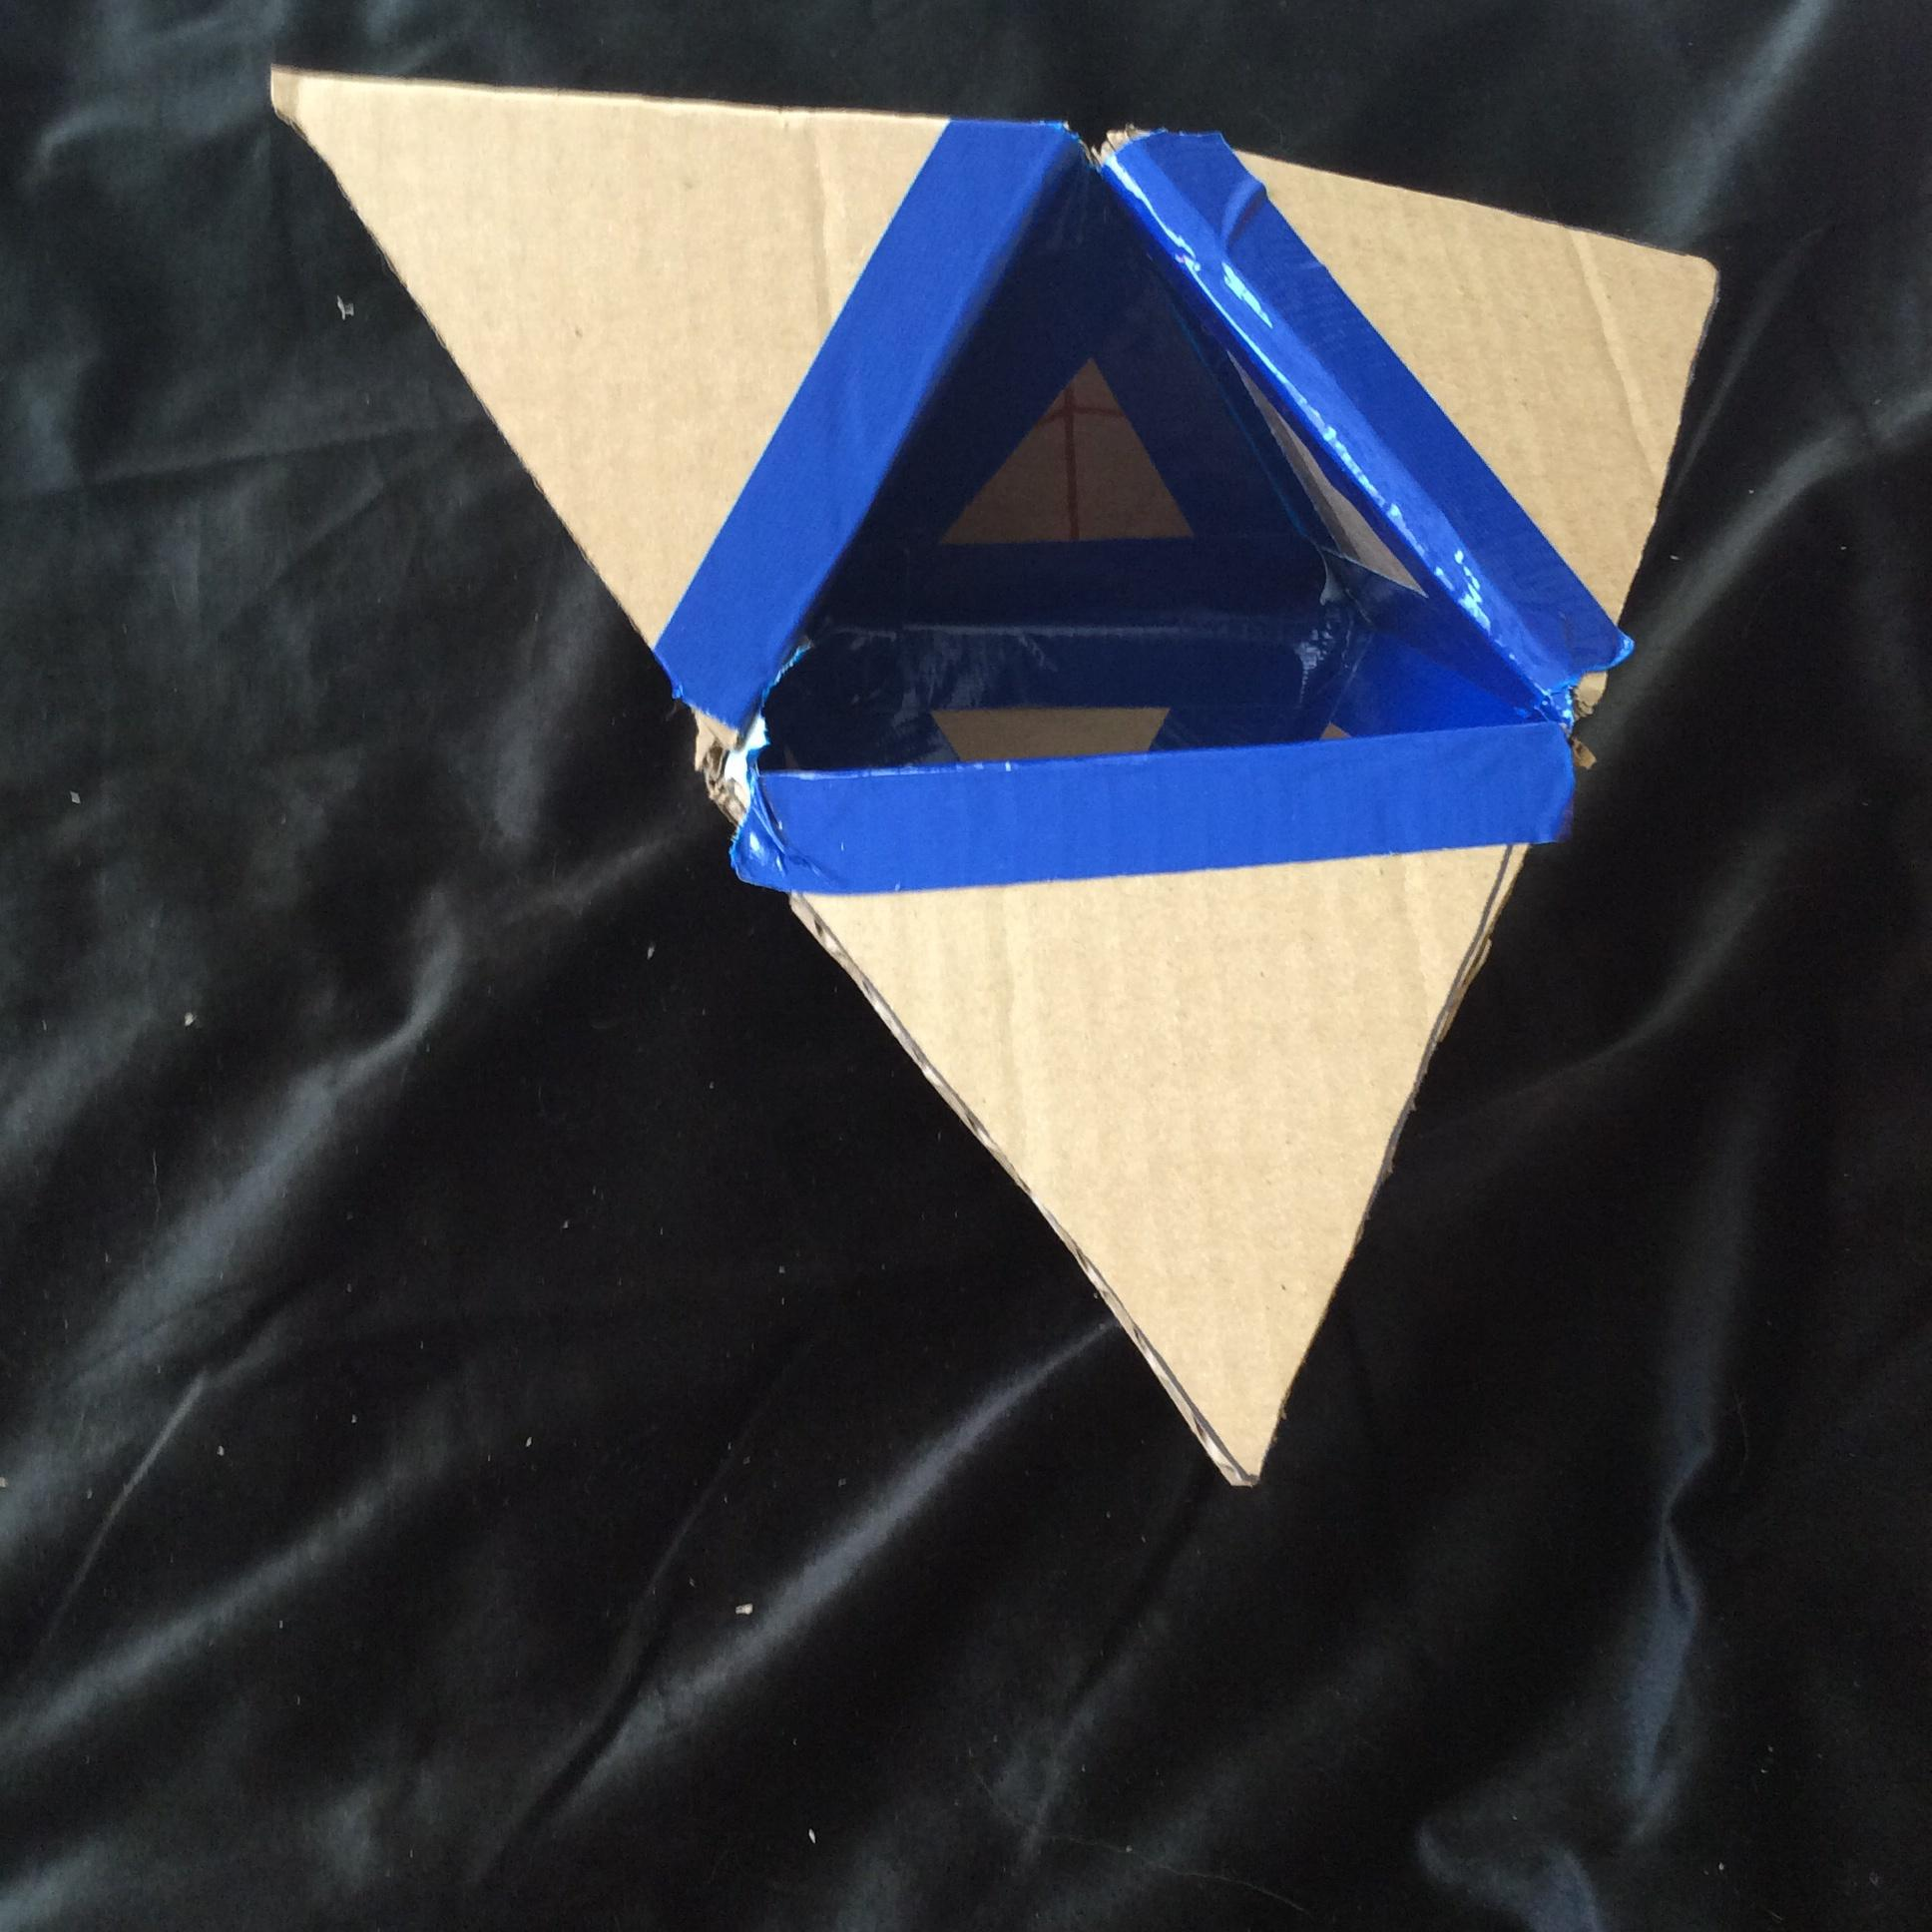
\includegraphics[width=4in]{figures/artboxassembly.jpg}
	\caption[artboxassembly]
	{Assemble into octahedron with three top triangles meeting in a tetrahedron top the octahedron.}
\end{figure}

\begin{figure}
	\centering
	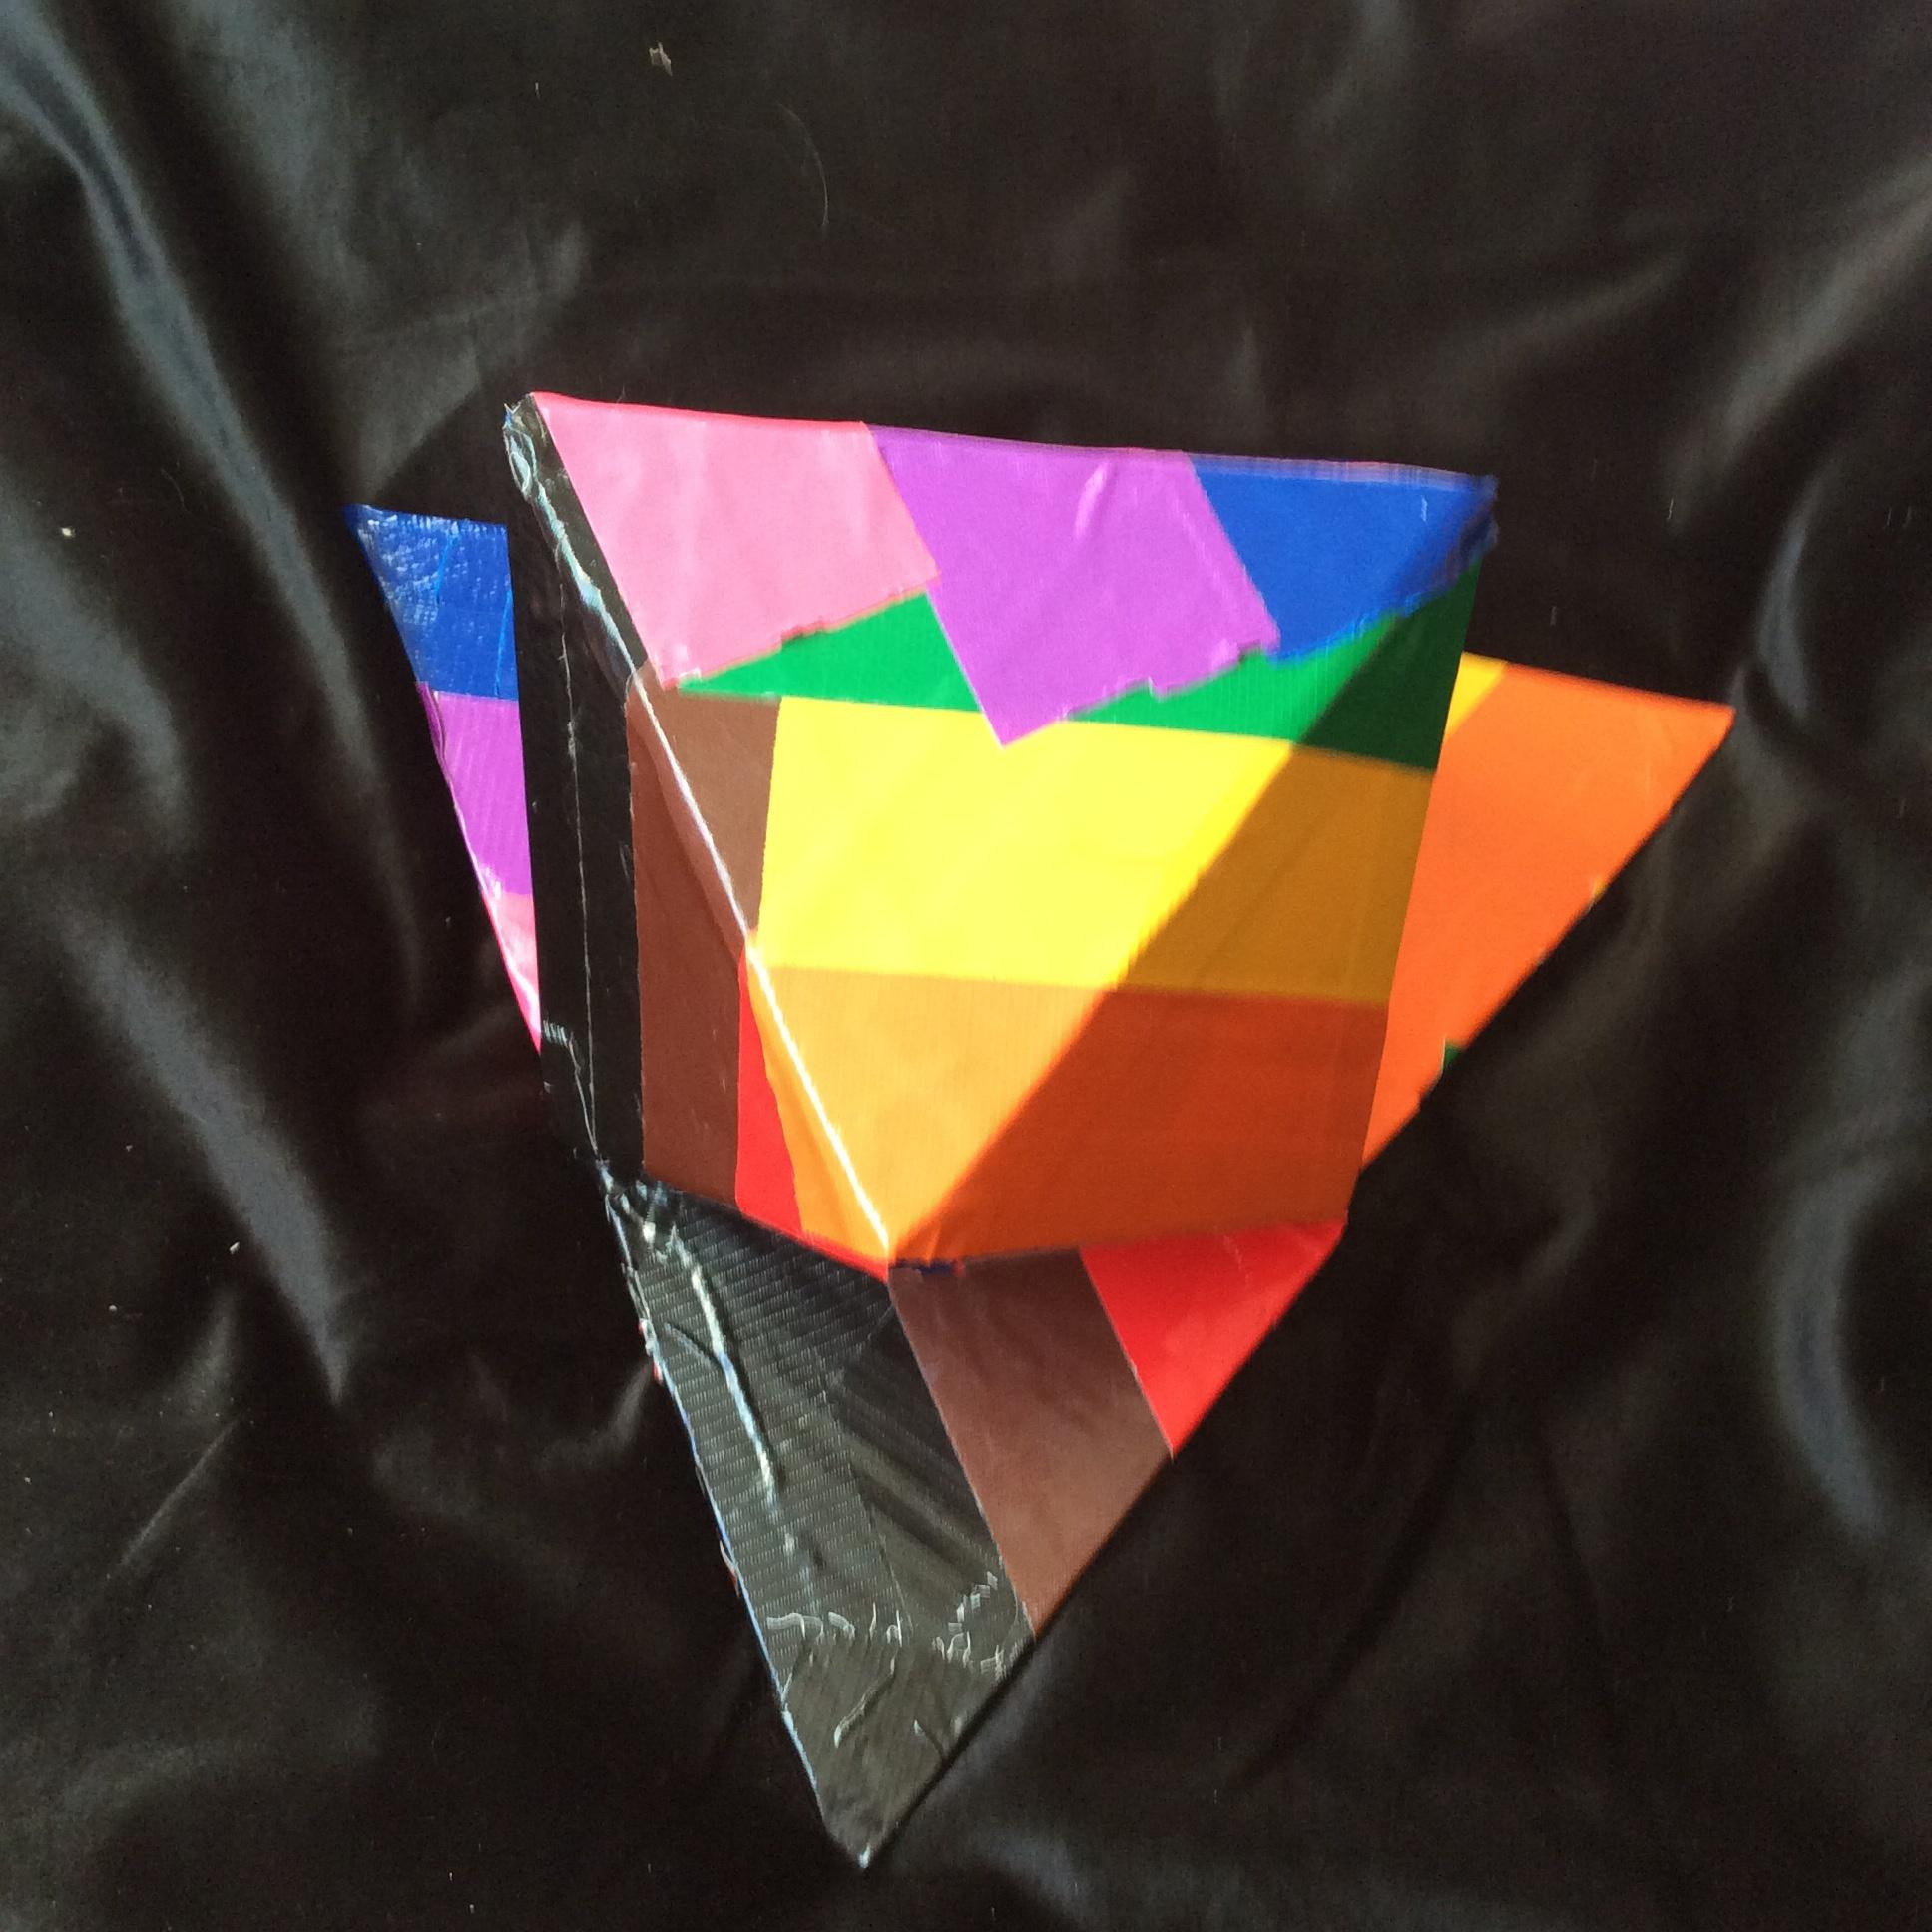
\includegraphics[width=4in]{figures/artboxrainbowskin.jpg}
	\caption[artboxrainbowskin]
	{Use all colors of duct tape to create rainbow skin effect as shown. This is the prototypical Trash Robot rainbow open brand after we add the mouth and googly eyes.} 
\end{figure}

\begin{figure}
	\centering
	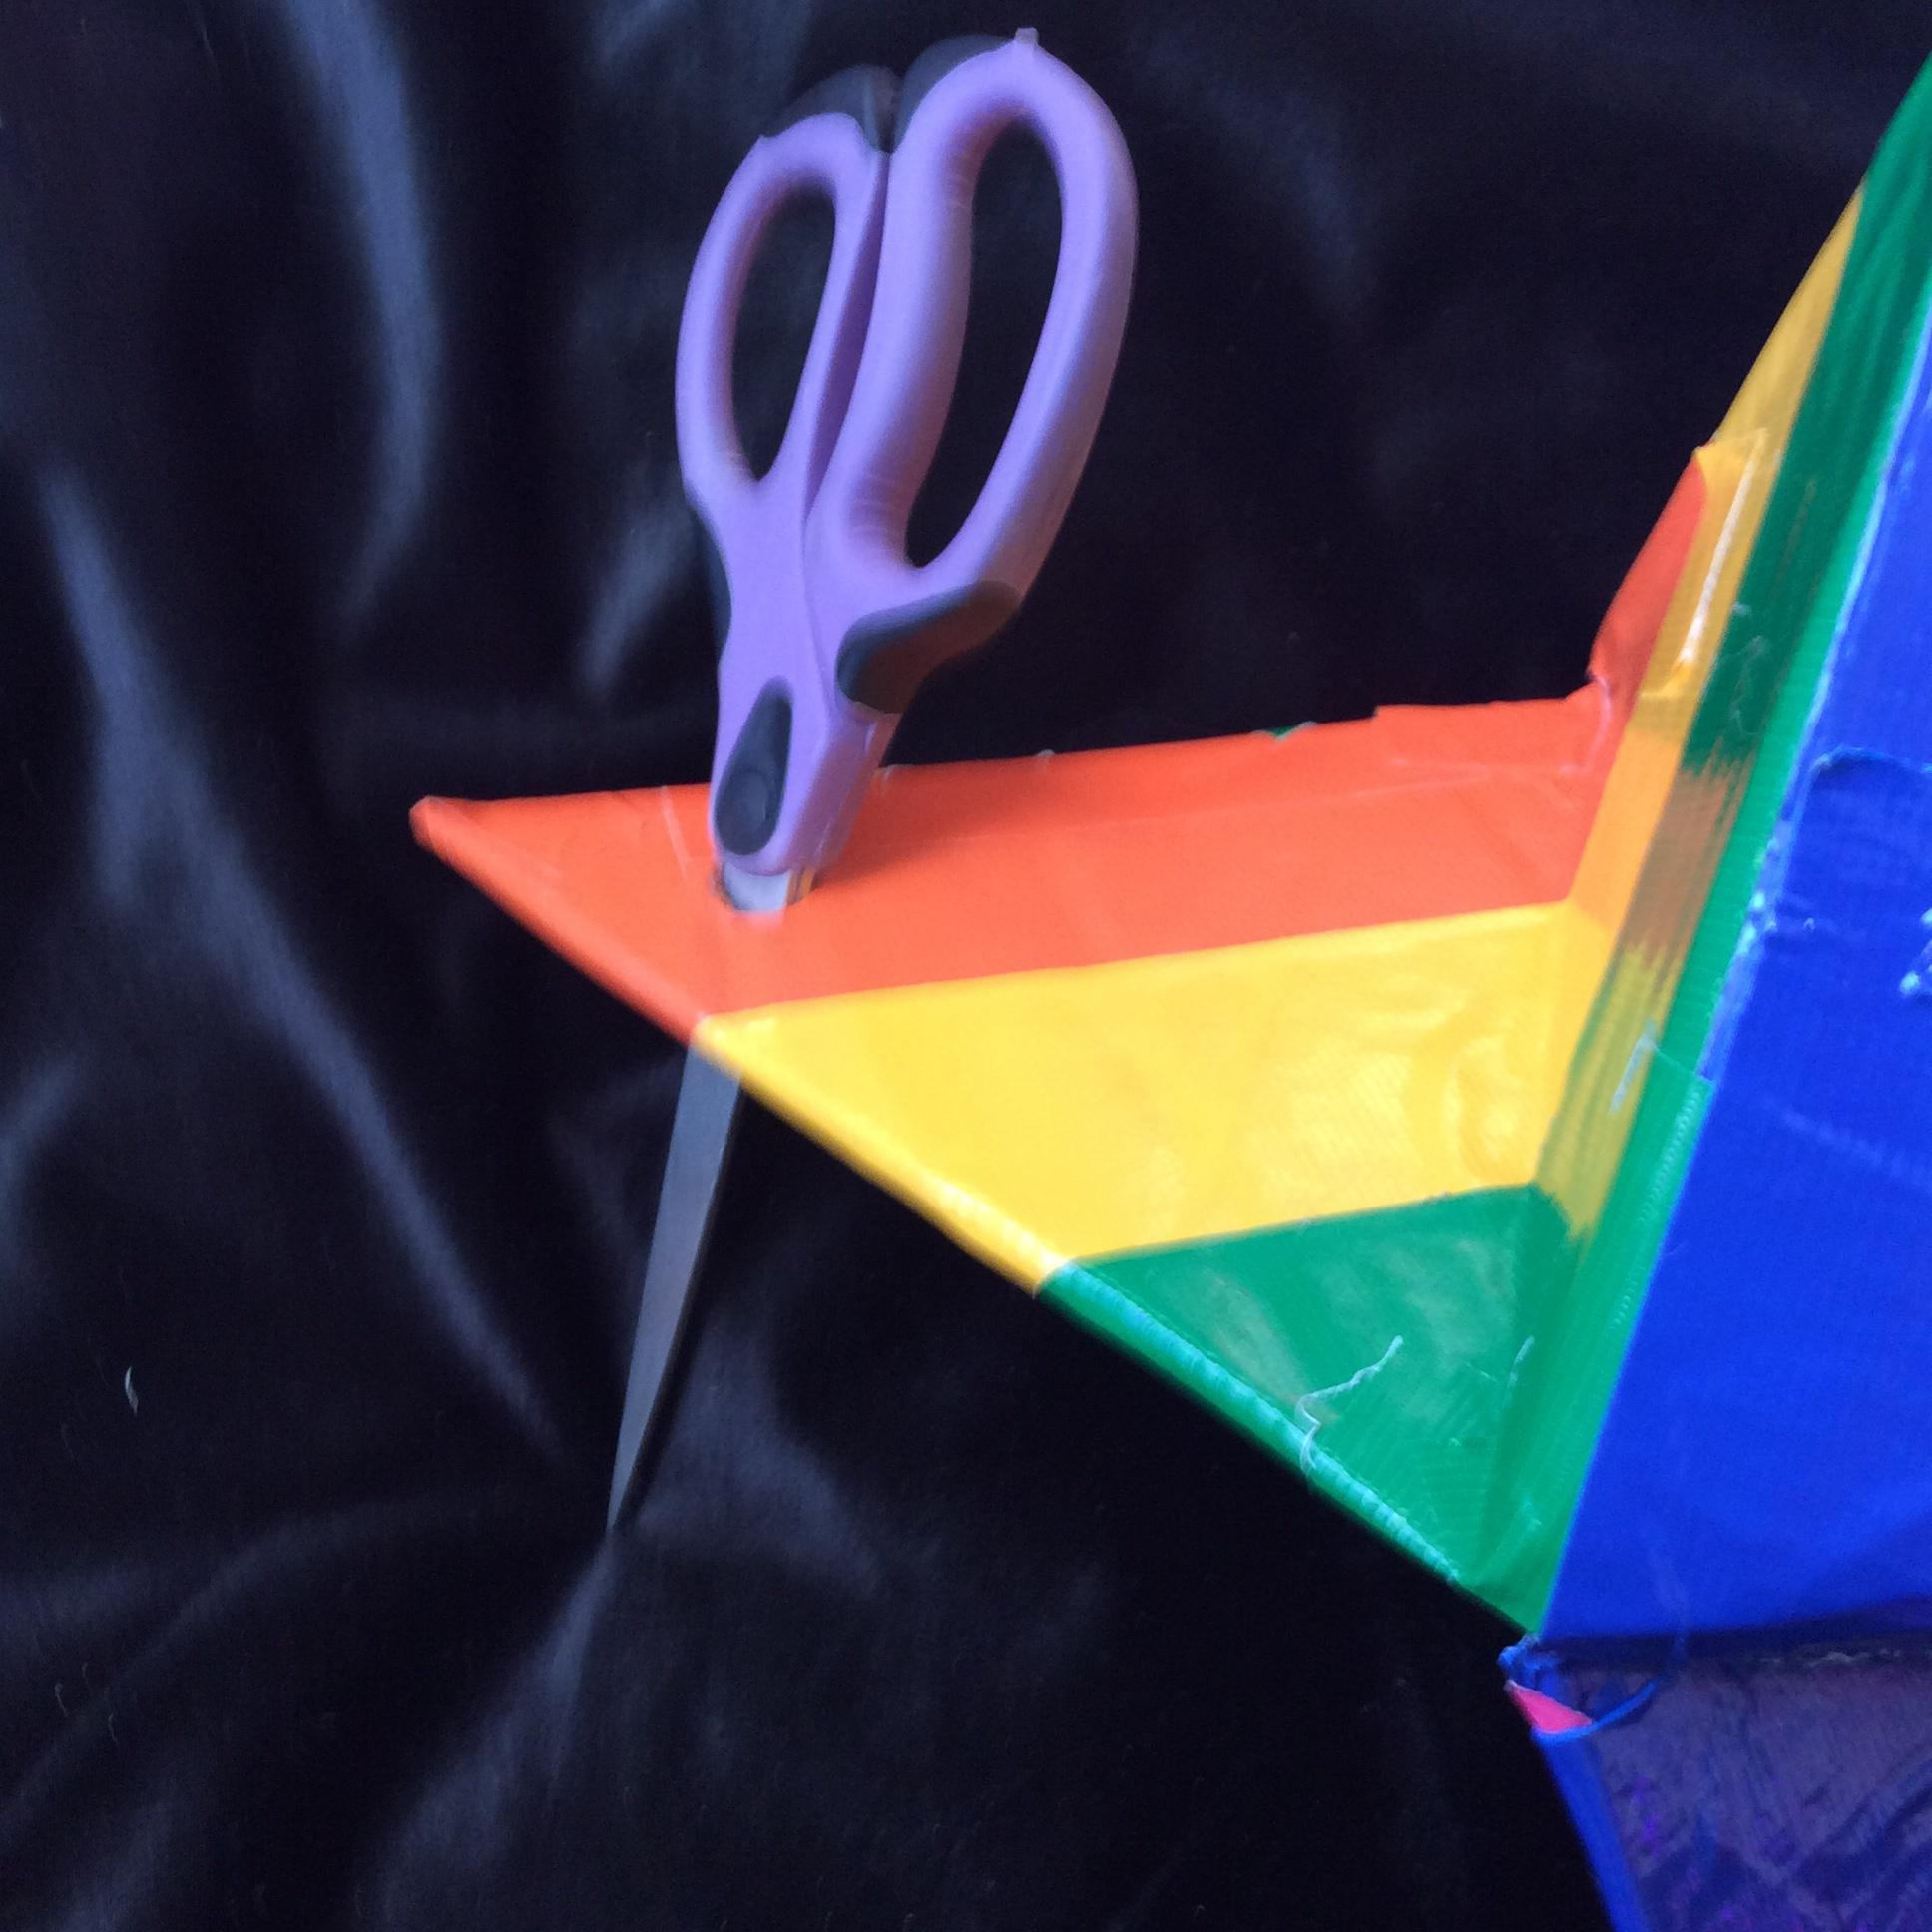
\includegraphics[width=4in]{figures/artboxhole.jpg}
	\caption[artboxhole]
	{Stab holes as shown in each of the top three triangles at the upper tips.}
\end{figure}

\begin{figure}
	\centering
	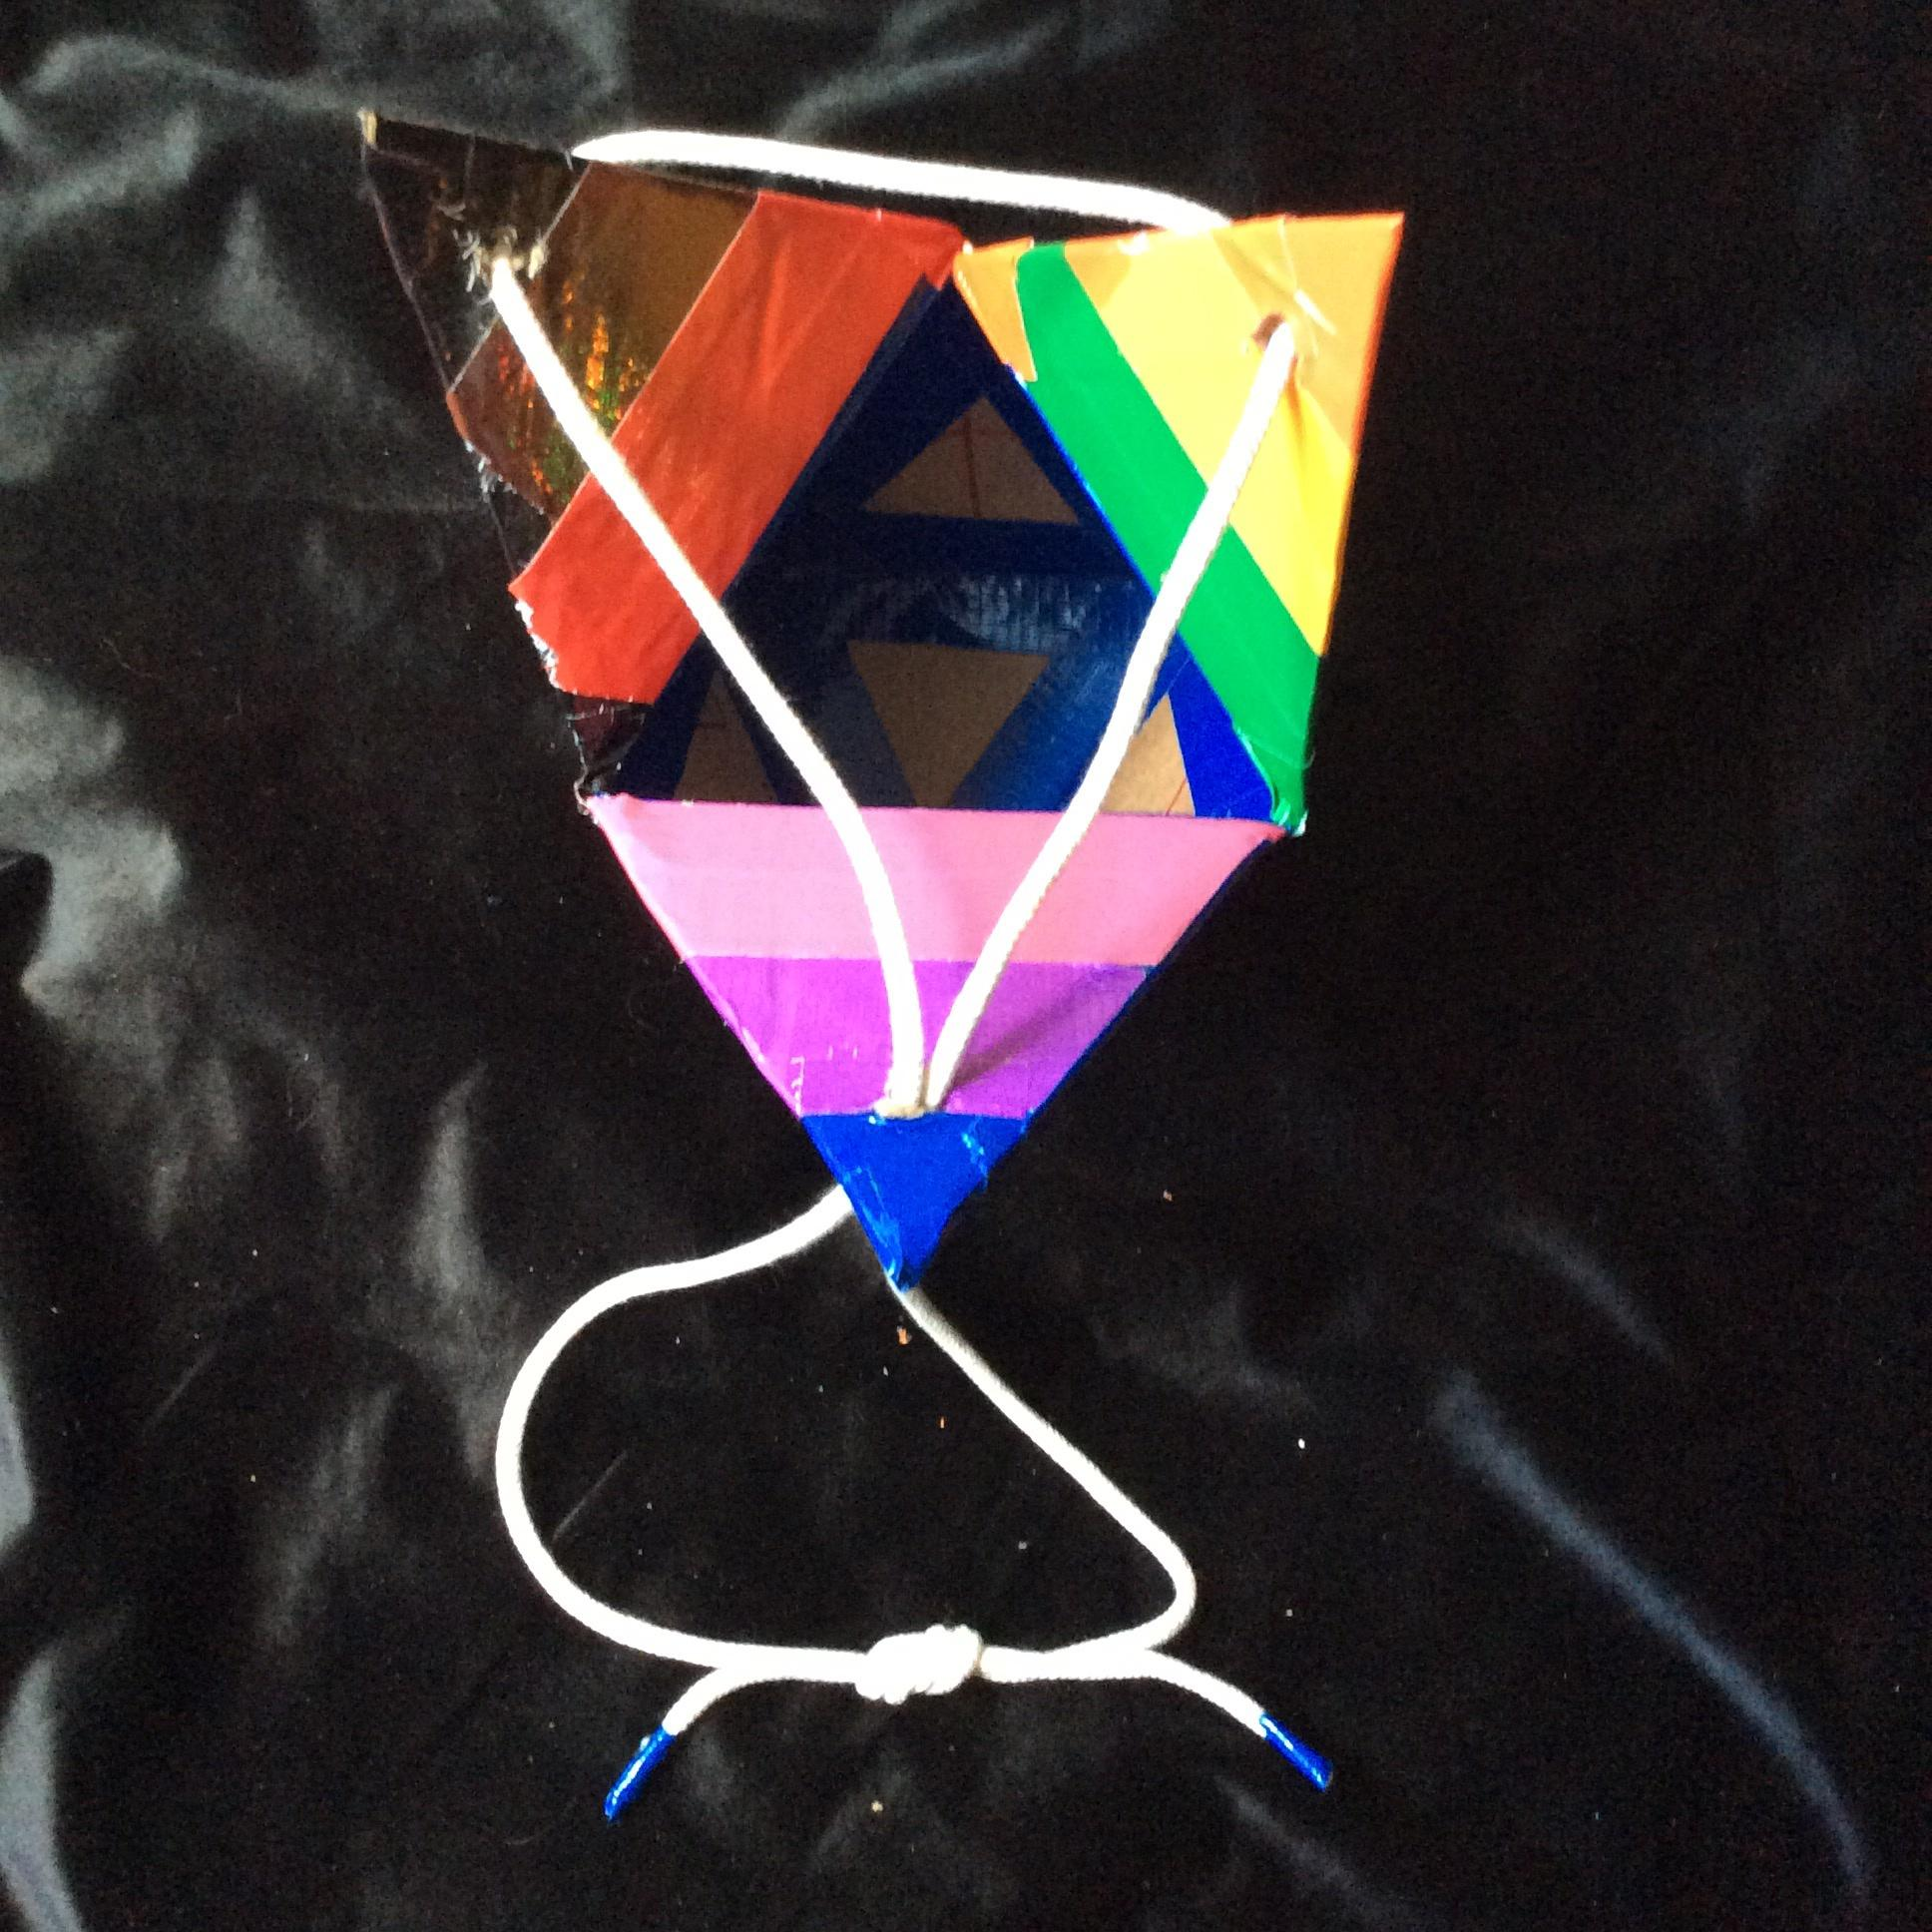
\includegraphics[width=4in]{figures/artboxtie.jpg}
	\caption[artboxtie]
	{Thread a Trash Tie, as described above, through the the holes as shown and tie a square knot.}
\end{figure}

\begin{figure}
	\centering
	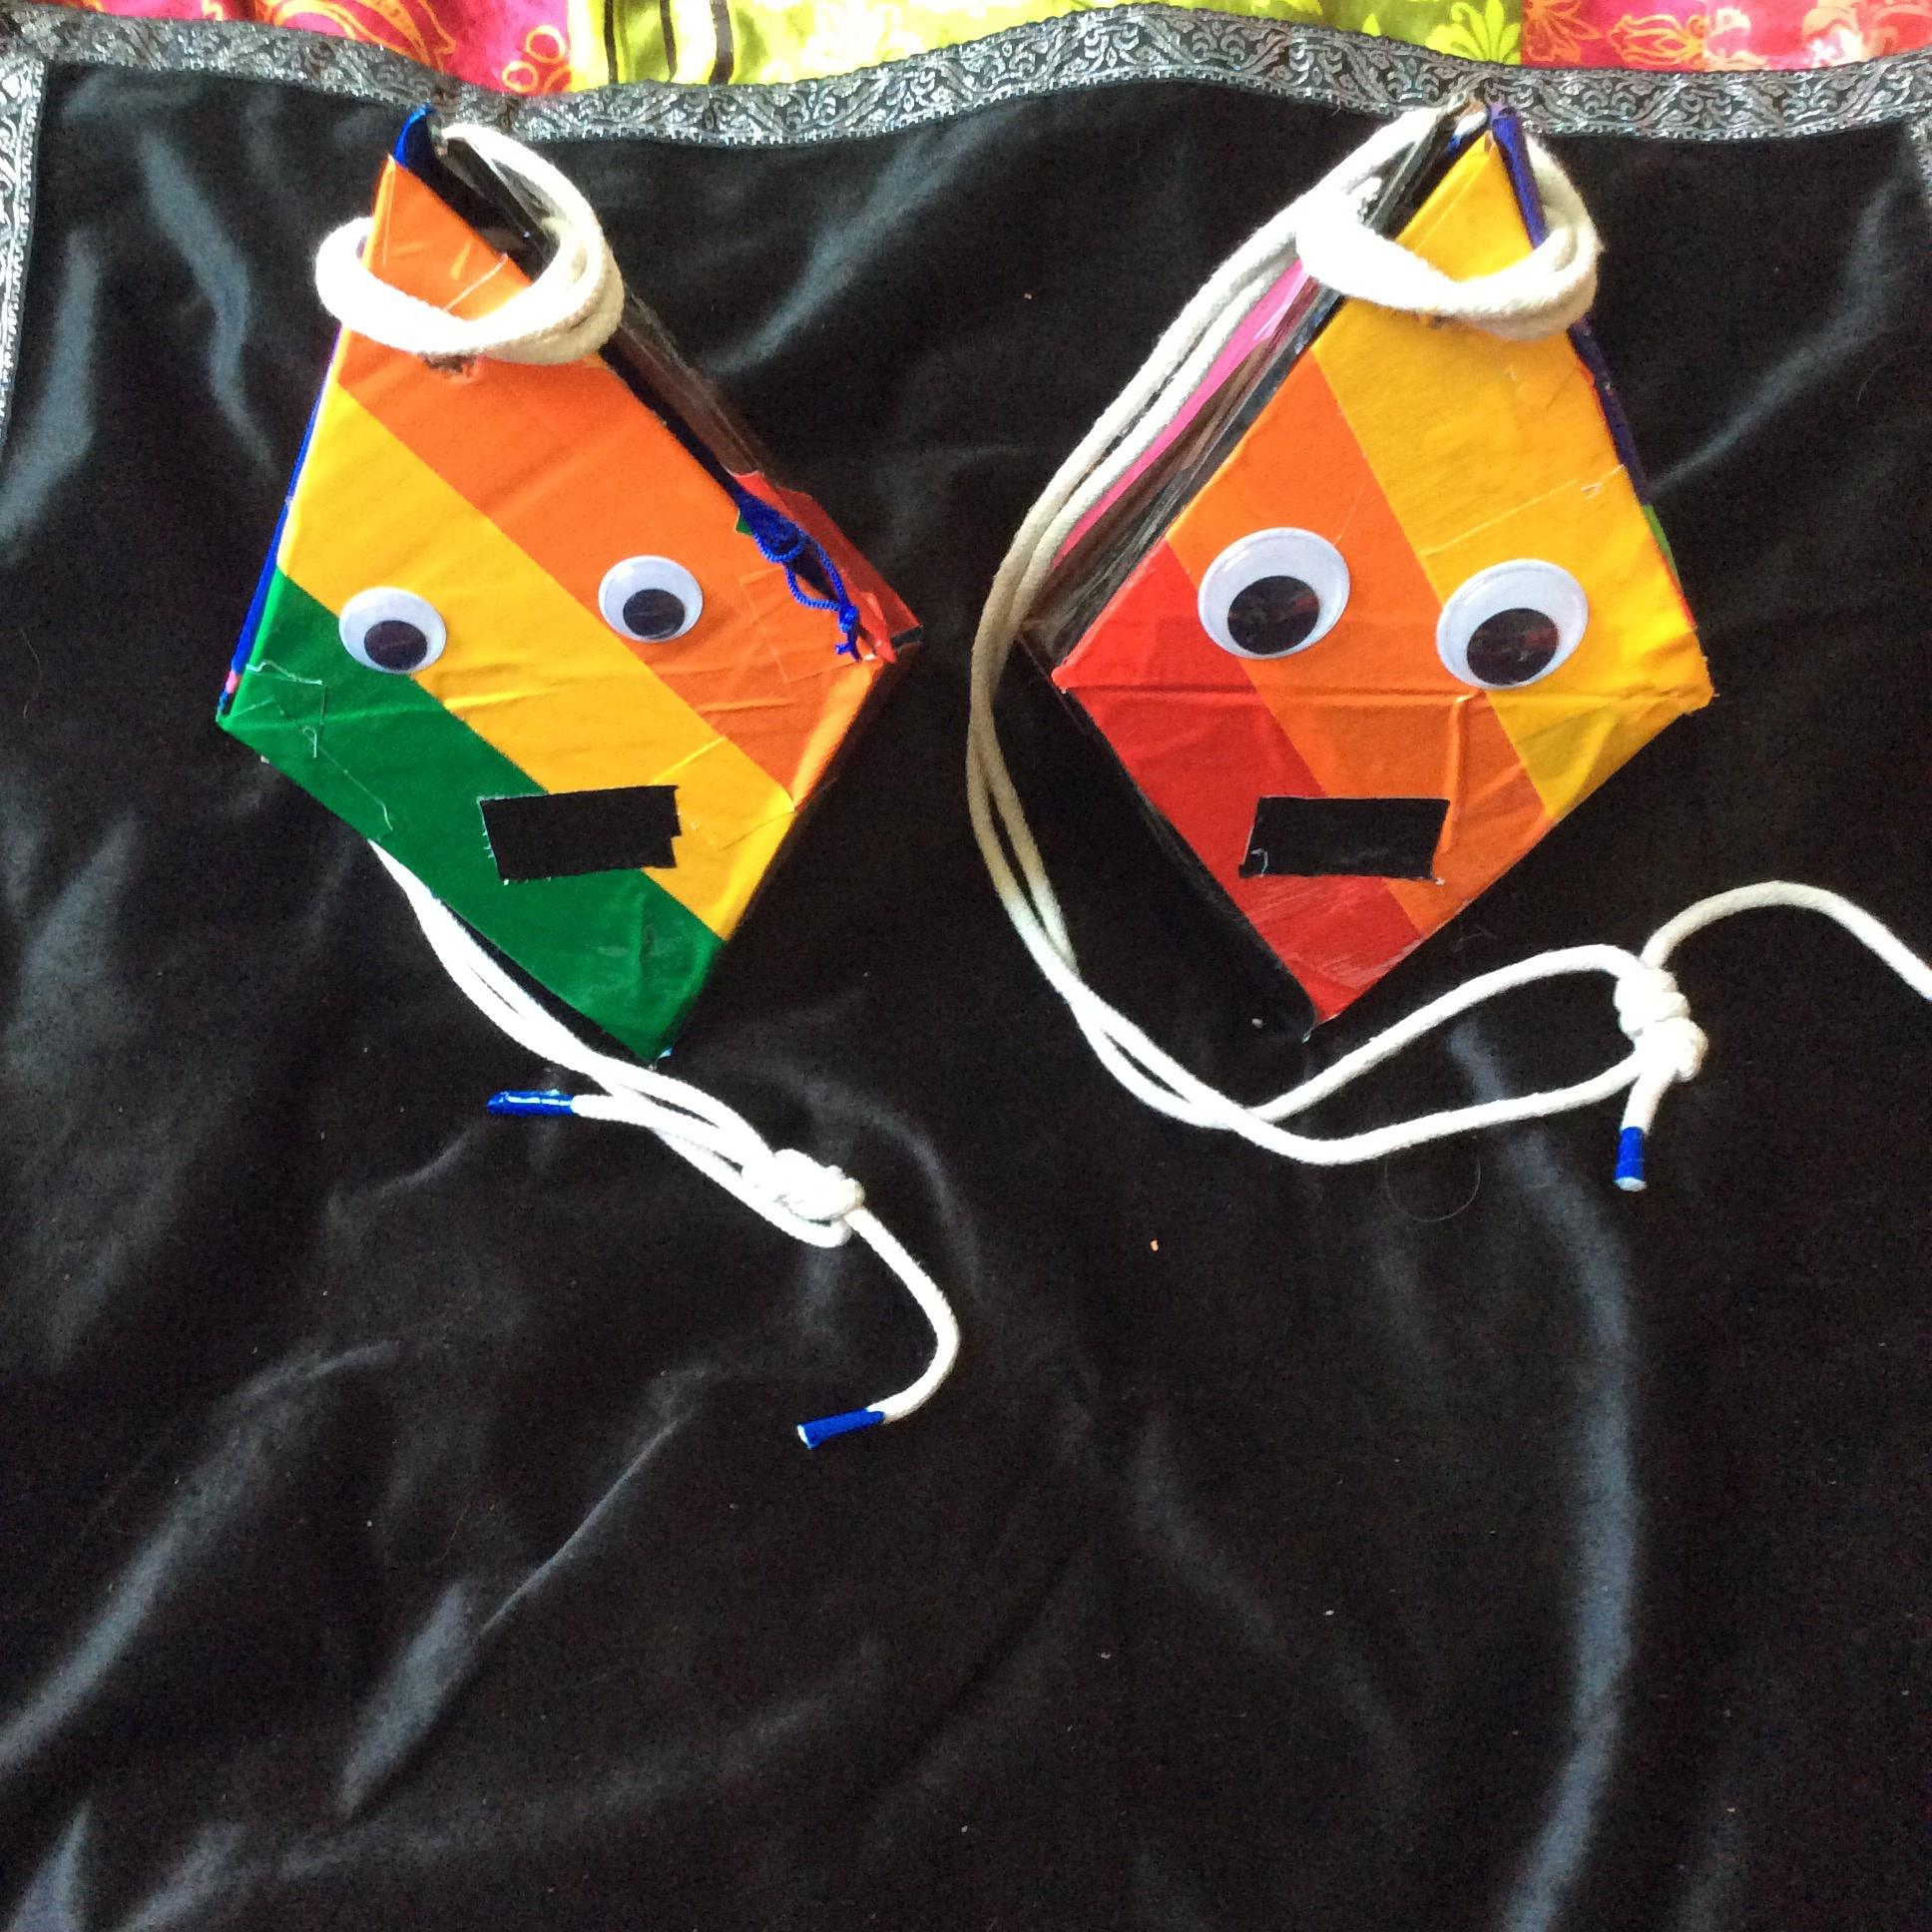
\includegraphics[width=4in]{figures/artboxcopy.jpg}
	\caption[artboxcopy]
	{Complete the box design with a black duct tape piece for the mouth and crookedly placed asymmetric googly eyes.  Multiple faces can all have the face design repeated.  Now we replicate all the contents, finding another sharpie, another box cutter, etc. and put a whole kit required to make another box in our box to use to make more boxes.  We also replicate the Tape Snake so that the new box has a Snake for replication, and pass some extra Trash Ties along for the next replication as well.}
\end{figure}

We will make millions of these to give away, share, or sell.  The can be freely shared in our Network without money or even barter and just used as needed for other Geometron constructions, but can always be sold to people not in the Network.

\subsection{Laser Cut Acrylic}

The Geometron workflow for creating .svg and .png files is designed among other things to make it as easy as possible to create files to use in commercial laser cutters.  These have been used both in the kind of laser cutter available in maker spaces and from the professional service at Ponoko.com(these require slightly different files).  

Laser neon green acrylic shapes in the basic Shape Set and the 6 inch Geometron ruler are key elements of our system, and replicate along with the rest of the ArtBox.  Making custom or specialized geometry tools like this is a very good metabusiness for Trash Robot.  We can sell the standard Shape Set, sell the Golden Triangle, the 6 inch Ruler, the Geometron Protractor, Penrose Tiles, custom spray stencils using the laser cut stencil font, and just custom arbitrary laser cut shapes for design clients.  

A good design target for custom spray stencils is the domain name which points to the local Geometron Raspberry Pi Server on the Street Network. 


Show each design. Link to global files.  How to use Dremel laser cutter, how to use Ponoko.  

\subsection{skeletron}

poles, geometry, tetrahedron, octahedron, icosahedron, tripods, flag poles, S Hooks, photos of constructions

\subsection{textiles}

the font. flags. Bags. Clothes.  Methodology. Fashion business on the street. all the layouts of the designs.  Waving the flag with the pole. Power of the flag to direct traffic to pages in the Network over the cardboard sign, legitimacy via the open brand.

\subsection{The icon token printer robot}

Build the brain. 

Build the controller. 

Build the mechanicals.  

Workflow:  image feeds, align, trace, share, print, bake, stamp, replicate, paint and sand, build into sets, share and sell, make pendants, stitch into clothing and accessories, make jewelry. Make more robots. Donate, share, and sell robots. 

The symbolic currency, creating sets, the sigil boards, sets as fashion, sets as symbolic currency which can mean \emph{anything}.  This symbolic currency goes back to the previous chapter, where we discuss the general idea of self-replicating sets. For any given set of generalized ``things'' in the sense of the previous chapter, each thing can be assigned a symbol.  That symbol can be traced into the robot code which drives the printer.  All those symbols can be stored as a token feed which is saved and shared with other users, who can then print them all out.  So an abstract set can always be represented by a collection of Geometron icon symbols shared over a network and also a collection of clay painted icon tokens, carried in a bag as described in the Textiles section of this chapter, and replicated using more clay without use of a robot.  So we can represent any self-replicating set with a set of symbols shared over both a local and global network and \emph{also} a collection of physical tokens in a bag which are like coins in a coin purse. Attractive and convenient coin purses which contain symbols representing a self-replicating set which themselves are self-replicating media can form the basis of a very powerful symbolic economy based on sets, networks, and symbols rather than numbers.  

The creation of a self-replicating symbolic currency which has both physical and digital versions is a fundamentally different type of currency than money.  Because it all self-replicates, the idea of property simply does not make sense, because the value of replication is reversed.  If I own a plot of land or a car, its value is based on how hard it is to replicate.  If it were possible to freely replicate a billion acres of the best land imaginable with warp drive to get to the best location, your million dollar plot of land will be worthless.  If someone builds a free car that grows naturally in a forest and runs on the sun, your 40,000 dollar gas car will be worthless.  But if you build a robot from trash to fabricate useful things, the more people copy the robot the more value there is in the whole network. If a billion people copy my robot, I can get a million of the cleverest makers in the world all improving the design, and what I end up using a few years from now light years beyond anything I could have even dreamed of.  So the more people replicate a free thing the \emph{more} that thing is worth to me, even as the creator of the thing.  This makes the way value works the opposite of property.  Value goes up with abundance rather than scarcity.  If we make the choice to value abundance, meaning the freeness of things, then that is what will end up with value.  But this replication also means that any numerical unit of value will very quickly break as the supply of value exceeds the total currency available again and again(essentially deflation).  

Some notes on the pi version, how this can be a pi driven robot.



\subsection{Arduino Generic Shield}

This is a stub.  It expands into many technologies but we document just the board and most basic of codes.  Future technologies will reference this.

\begin{verbatim}
Trash Robot = {
    ArtBox,
    Trash Tie,
    Tape Snake,
    Token Printer,
    Terminal,
    Brand,
    Textile,
    Shop,
    skeletron,
    constructions
}
\end{verbatim}
    
\begin{verbatim}
constructions = {
    duct tape, 
    cardboard, 
    trash ties, 
    HDPE sheets
}
\end{verbatim}
\begin{verbatim}
shop = {
    ArtBox purse, 
    Trash Robot branded clothes, 
    laser cut acrylic, 
    token printer kits,
    tokens,
    pendants,
    printed bottle caps,
    terminal install
}
\end{verbatim}

\begin{verbatim}
laser cut acrylic = {
    golden triangles, 
    penrose tiles, 
    full set, 
    ruler,
    protractor,
    custom shape,
    spray stencils
}
\end{verbatim}

\begin{verbatim}
printer = {
    brain,
    controller,
    mechanicals,
    workflow
}
\end{verbatim}

\begin{verbatim}
    printer workflow = {
        build, share, sell, use printers, following instructions on scrolls on Geometron
        use Geometron server to follow the rest of this workflow: 
        image feeds,
        aligner,
        trace,
        share feed with other users, save, copy, paste, share share share!!
        load code into Arduino, print in clay tablet, bake it, sell or give away or use
        use print to create stamp, sell or give away or use,
        use stamp to create both coin-like tokens and pendants, stamping in clay, baking, using paint pen and sanding flat, sell, trade, or wear
    }
\end{verbatim}
    